\documentclass{vkr}
\usepackage[english, russian]{babel} % переносы
\usepackage{graphicx} % для вставки картинок
\graphicspath{{images/}} % путь к изображениям
\usepackage[hidelinks]{hyperref}
\usepackage{float} % определяет метод H для рисунка с переносом на следующую страницу, ели не помещается
\usepackage{pdflscape}
\addto{\captionsrussian}{\renewcommand{\refname}{СПИСОК ИСПОЛЬЗОВАННЫХ ИСТОЧНИКОВ}}
\usepackage{xltabular} % для вставки таблиц
\usepackage{makecell}
\renewcommand\theadfont{} % шрифт в /thead
\usepackage{array} % для определения новых типов столбцов таблиц
\newcolumntype{T}{>{\centering\arraybackslash}X} % новый тип столбца T - автоматическая ширина столбца с выравниванием по центру
\newcolumntype{R}{>{\raggedleft\arraybackslash}X} % новый тип столбца R - автоматическая ширина столбца с выравниванием по правому краю
\newcolumntype{C}[1]{>{\centering\let\newline\\\arraybackslash\hspace{0pt}}m{#1}} % новый тип столбца C - фиксированная ширина столбца с выравниванием по центру
\newcolumntype{r}[1]{>{\raggedleft\arraybackslash}p{#1}} % новый тип столбца r - фиксированная ширина столбца с выравниванием по правому краю
\newcommand{\centrow}{\centering\arraybackslash} % командой \centrow можно центрировать одну ячейку (заголовок) в столбце типа X или p, оставив в оcтальных ячейках другой тип выравнивания
\newcommand{\finishhead}{\endhead\hline\endlastfoot}
\newcommand{\continuecaption}[1]{\caption*{#1}\\ \hline }
\usepackage{etoolbox}
\AtBeginEnvironment{xltabular}{\refstepcounter{tablecnt}} % подсчет таблиц xltabular, обычные таблицы подсчитываются в классе

\usepackage[tableposition=top]{caption} % подпись таблицы вверху
\captionsetup{strut=off}
\setlength{\intextsep}{0pt} % Vertical space above & below [h] floats
\setlength{\textfloatsep}{0pt} % Vertical space below (above) [t] ([b]) floats
\DeclareCaptionLabelFormat{gostfigure}{Рисунок #2} %подпись рисунка
\DeclareCaptionLabelFormat{gosttable}{Таблица #2} %подпись таблицы
\DeclareCaptionLabelSeparator{gost}{~--~} %разделитель в рисунках и таблицах
\captionsetup{labelsep=gost}
\captionsetup[figure]{aboveskip=10pt,belowskip=4mm,justification=centering,labelformat=gostfigure} % настройка подписи рисунка
\captionsetup[table]{font={stretch=1.41},skip=0pt,belowskip=0pt,aboveskip=8.5pt,singlelinecheck=off,labelformat=gosttable} % настройка подписи таблицы

\setlength{\LTpre}{8mm} % отступ сверху таблицы
\setlength{\LTpost}{6mm} % отступ снизу таблицы

\usepackage{enumitem}
\setlist{nolistsep,wide=\parindent,itemindent=*} % отступы вокруг списков, выравнивание с учетом разделителя

\usepackage{color} %% это для отображения цвета в коде
\usepackage{listings} %% листинги кода
\setmonofont[Scale=0.7]{Verdana} % моноширный шрифт для листинга

\definecolor{codegreen}{rgb}{0,0.6,0}
\definecolor{codegray}{rgb}{0.5,0.5,0.5}
\definecolor{codepurple}{rgb}{0.58,0,0.82}

\lstset{ %
language=C,                 % выбор языка для подсветки (здесь это С)
numbers=left,               % где поставить нумерацию строк (слева\справа)
numberstyle=\tiny,           % размер шрифта для номеров строк
stepnumber=1,                   % размер шага между двумя номерами строк
numbersep=5pt,                % как далеко отстоят номера строк от подсвечиваемого кода
commentstyle=\color{codegreen},
keywordstyle=\color{magenta},
numberstyle=\tiny\color{codegray},
stringstyle=\color{codepurple},
basicstyle=\linespread{0.95}\ttfamily,
backgroundcolor=\color{white}, % цвет фона подсветки - используем \usepackage{color}
showspaces=false,            % показывать или нет пробелы специальными отступами
showstringspaces=false,      % показывать или нет пробелы в строках
showtabs=false,             % показывать или нет табуляцию в строках
frame=single,              % рисовать рамку вокруг кода
tabsize=2,                 % размер табуляции по умолчанию равен 2 пробелам
captionpos=t,              % позиция заголовка вверху [t] или внизу [b] 
breaklines=true,           % автоматически переносить строки (да\нет)
breakatwhitespace=false, % переносить строки только если есть пробел
escapeinside={\%*}{*)}   % если нужно добавить комментарии в коде
}

\makeatletter % чтобы допускались русские комментарии в листингах
\lst@InputCatcodes
\def\lst@DefEC{%
 \lst@CCECUse \lst@ProcessLetter
  ^^80^^81^^82^^83^^84^^85^^86^^87^^88^^89^^8a^^8b^^8c^^8d^^8e^^8f%
  ^^90^^91^^92^^93^^94^^95^^96^^97^^98^^99^^9a^^9b^^9c^^9d^^9e^^9f%
  ^^a0^^a1^^a2^^a3^^a4^^a5^^a6^^a7^^a8^^a9^^aa^^ab^^ac^^ad^^ae^^af%
  ^^b0^^b1^^b2^^b3^^b4^^b5^^b6^^b7^^b8^^b9^^ba^^bb^^bc^^bd^^be^^bf%
  ^^c0^^c1^^c2^^c3^^c4^^c5^^c6^^c7^^c8^^c9^^ca^^cb^^cc^^cd^^ce^^cf%
  ^^d0^^d1^^d2^^d3^^d4^^d5^^d6^^d7^^d8^^d9^^da^^db^^dc^^dd^^de^^df%
  ^^e0^^e1^^e2^^e3^^e4^^e5^^e6^^e7^^e8^^e9^^ea^^eb^^ec^^ed^^ee^^ef%
  ^^f0^^f1^^f2^^f3^^f4^^f5^^f6^^f7^^f8^^f9^^fa^^fb^^fc^^fd^^fe^^ff%
  ^^^^20ac^^^^0153^^^^0152%
  % Basic Cyrillic alphabet coverage
  ^^^^0410^^^^0411^^^^0412^^^^0413^^^^0414^^^^0415^^^^0416^^^^0417%
  ^^^^0418^^^^0419^^^^041a^^^^041b^^^^041c^^^^041d^^^^041e^^^^041f%
  ^^^^0420^^^^0421^^^^0422^^^^0423^^^^0424^^^^0425^^^^0426^^^^0427%
  ^^^^0428^^^^0429^^^^042a^^^^042b^^^^042c^^^^042d^^^^042e^^^^042f%
  ^^^^0430^^^^0431^^^^0432^^^^0433^^^^0434^^^^0435^^^^0436^^^^0437%
  ^^^^0438^^^^0439^^^^043a^^^^043b^^^^043c^^^^043d^^^^043e^^^^043f%
  ^^^^0440^^^^0441^^^^0442^^^^0443^^^^0444^^^^0445^^^^0446^^^^0447%
  ^^^^0448^^^^0449^^^^044a^^^^044b^^^^044c^^^^044d^^^^044e^^^^044f%
  ^^^^0401^^^^0451%
  %%%
  ^^00}
\lst@RestoreCatcodes
\makeatother


% Режим шаблона (должен быть включен один из трех)
%\ВКРtrue
\Практикаtrue
%\Курсоваяtrue

\newcommand{\Дисциплина}{<<Проектирование и архитектура программных систем>>} % для курсовой
\newcommand{\КодСпециальности}{09.03.04} % Курсовая
\newcommand{\Специальность}{Программная инженерия} % Курсовая
\newcommand{\Тема}{Интеллектуальная система распознавания объектов по цветовым} % ВКР Курсовая
\newcommand{\ТемаВтораяСтрока}{характеристикам на основе нечетких нейронных сетей}
\newcommand{\ГдеПроводитсяПрактика}{ООО «Предприятие ВТИ-Сервис»} % для практики
\newcommand{\РуководительПрактПредпр}{Куркина А. В.} % для практики
\newcommand{\ДолжнРуководительПрактПредпр}{директор} % для практики
\newcommand{\РуководительПрактУнивер}{Чаплыгин А. А.} % для практики
\newcommand{\ДолжнРуководительПрактУнивер}{к.т.н. доцент} % для практики
\newcommand{\Автор}{В.В. Тягунов}
\newcommand{\АвторРод}{Тягунова В.В..}
\newcommand{\АвторПолностьюРод}{Тягунова Владимира Вячеславовича} % для практики
\newcommand{\Шифр}{20-06-0149}
\newcommand{\Курс}{4} % для практики
\newcommand{\Группа}{ПО-02б}
\newcommand{\Руководитель}{Р.А. Томакова} % для ВКР и курсовой
\newcommand{\Нормоконтроль}{А. А. Чаплыгин} % для ВКР
\newcommand{\ЗавКаф}{А. В. Малышев} % для ВКР
\newcommand{\ДатаПриказа}{«07» апреля 2023~г.} % для ВКР
\newcommand{\НомерПриказа}{1505-с} % для ВКР
\newcommand{\СрокПредоставления}{«13» июня 2023~г.} % для ВКР, курсового	

\begin{document}
\maketitle
\ifПрактика{}\else{
   \newpage
\begin{center}
\large\textbf{Минобрнауки России}

\large\textbf{Юго-Западный государственный университет}
\vskip 1em
\normalsize{Кафедра программной инженерии}
\vskip 1em
\ifВКР{
        \begin{flushright}
        \begin{tabular}{p{.4\textwidth}}
        \centrow УТВЕРЖДАЮ: \\
        \centrow Заведующий кафедрой \\
        \hrulefill \\
        \setarstrut{\footnotesize}
        \centrow\footnotesize{(подпись, инициалы, фамилия)}\\
        \restorearstrut
        «\underline{\hspace{1cm}}»
        \underline{\hspace{3cm}}
        20\underline{\hspace{1cm}} г.\\
        \end{tabular}
        \end{flushright}
        }\fi
\end{center}
\vspace{1em}
  \begin{center}
  \large
\ifВКР{
ЗАДАНИЕ НА ВЫПУСКНУЮ КВАЛИФИКАЦИОННУЮ РАБОТУ
  ПО ПРОГРАММЕ БАКАЛАВРИАТА}
  \else
ЗАДАНИЕ НА КУРСОВУЮ РАБОТУ (ПРОЕКТ)
\fi
\normalsize
  \end{center}
\vspace{1em}
{\parindent0pt
  Студента \АвторРод, шифр\ \Шифр, группа \Группа
  
1. Тема «\Тема\ \ТемаВтораяСтрока»
\ifВКР{
утверждена приказом ректора ЮЗГУ от \ДатаПриказа\ № \НомерПриказа
}\fi.

2. Срок предоставления работы к защите \СрокПредоставления

3. Исходные данные для создания программной системы:

3.1. Перечень решаемых задач:}

\renewcommand\labelenumi{\theenumi)}

\begin{enumerate}
\item проанализировать IT-инфраструктуру предприятия;
\item  разработать концептуальную модель системы управления IT-ин\-фра\-струк\-турой предприятия на основе подхода к управлению и организации ИТ-услуг ITSM;
\item спроектировать программную систему управления IT-ин\-фра\-струк\-турой предприятия;
\item сконструировать и протестировать программную систему управления IT-инфраструктурой предприятия.
\end{enumerate}

{\parindent0pt
  3.2. Входные данные и требуемые результаты для программы:}

\begin{enumerate}
\item Входными данными для программной системы являются: данные
справочников комплектующих, конфигураций, ПО, критериев качества SLA,
ИТ-услуг, департаментов компании; технические данные ИТ-ресурсов; данные входящих заявок на ИТ-ресурсы; данные запросов поставщикам на комплектующие.
\item Выходными данными для программной системы являются: сформированные заявки на обслуживание ИТ-ресурсов; сформированные запросы на
закупку комплектующих; сведения о выполненных работах по заявкам; статусы заявок; выходные отчеты (инфографика) – по качеству услуг, по состоянию ИТ-ресурсов, по деятельности ИТ-отдела, по стоимости обслуживания
ИТ-ресурсов, воронка заявок.
\end{enumerate}

{\parindent0pt

  4. Содержание работы (по разделам):
  
  4.1. Введение
  
  4.1. Анализ предметной области
  
4.2. Техническое задание: основание для разработки, назначение разработки,
требования к программной системе, требования к оформлению документации.

4.3. Технический проект: общие сведения о программной системе, проект
данных программной системы, проектирование архитектуры программной системы, проектирование пользовательского интерфейса программной системы.

4.4. Рабочий проект: спецификация компонентов и классов программной системы, тестирование программной системы, сборка компонентов программной системы.

4.5. Заключение

4.6. Список использованных источников

5. Перечень графического материала:

\списокПлакатов

\vskip 2em
\begin{tabular}{p{6.8cm}C{3.8cm}C{4.8cm}}
Руководитель \ifВКР{ВКР}\else работы (проекта) \fi & \lhrulefill{\fill} & \fillcenter\Руководитель\\
\setarstrut{\footnotesize}
& \footnotesize{(подпись, дата)} & \footnotesize{(инициалы, фамилия)}\\
\restorearstrut
Задание принял к исполнению & \lhrulefill{\fill} & \fillcenter\Автор\\
\setarstrut{\footnotesize}
& \footnotesize{(подпись, дата)} & \footnotesize{(инициалы, фамилия)}\\
\restorearstrut
\end{tabular}
}

\renewcommand\labelenumi{\theenumi.}

   \abstract{РЕФЕРАТ}

Объем работы равен \formbytotal{lastpage}{страниц}{е}{ам}{ам}. Работа содержит \formbytotal{figurecnt}{иллюстраци}{ю}{и}{й}, \formbytotal{tablecnt}{таблиц}{у}{ы}{}, \arabic{bibcount} библиографических источников и \formbytotal{числоПлакатов}{лист}{}{а}{ов} графического материала. Количество приложений – 2. Графический материал представлен в приложении А. Фрагменты исходного кода представлены в приложении Б.

Перечень ключевых слов: компьютерное зрение, язык Python, средства MATLAB, приложение, нечёткая нейронная сеть, система, информатизация, автоматизация, информационные технологии, классы, ANFIS, база данных, компонент, нечёткая логика, модуль, сущность, метод, пользователь, нейросеть, стационарное приложение.

Объектом разработки является стационарное приложение,  обеспечивающее возможность распознавания объектов по цветовым характеристикам на основе нечётких нейронных сетей.

Целью выпускной квалификационной работы является проведение глубокого анализа и исследования передовых технологий в области компьютерного зрения и искусственного интеллекта. Работа фокусируется на применении нечётких нейронных сетей, что позволяет значительно повысить точность и эффективность процесса распознавания объектов.

В ходе разработки приложения был выполнен ряд ключевых шагов: определение и структурирование основных сущностей через создание информационных модулей, применение классов и методов для управления данными в соответствии с предметной областью и для обеспечения надёжности функционирования приложения. Была спроектирована архитектура нечёткой нейронной сети и базы данных, а также разработан пользовательский интерфейс, облегчающий взаимодействие с приложением.

Для создания веб-сайта были использованы возможности языка программирования Python в сочетании с инструментарием библиотек MATLAB, что позволило реализовать необходимые функциональные возможности.

\selectlanguage{english}
\abstract{ABSTRACT}

The amount of work is equal to \formbytotal{lastpage} pages. The work contains \formbytotal{figurecnt} illustrations, \formbytotal{tablecnt} tables, \arabic{bibcount} bibliographic sources and \formbytotal{числоПлакатов} sheets of graphic material. Number of applications – 2. Graphic material is presented in Appendix A. Source code fragments are presented in Appendix B.

List of keywords: computer vision, Python language, MATLAB tools, application, fuzzy neural network, system, informatization, automation, information technology, classes, ANFIS, database, component, fuzzy logic, module, entity, method, user, neural network, stationary application.

The object of development is a stationary application that provides the ability to recognize objects by color characteristics based on fuzzy neural networks.

The purpose of the final qualifying work is to conduct in-depth analysis and research of advanced technologies in the field of computer vision and artificial intelligence. The work focuses on the use of fuzzy neural networks, which can significantly improve the accuracy and efficiency of the object recognition process.

During the development of the application, a number of key steps were completed: defining and structuring the main entities through the creation of information modules, using classes and methods to manage data in accordance with the subject area and to ensure the reliability of the application. The architecture of the fuzzy neural network and database was designed, and a user interface was developed to facilitate interaction with the application.

To create the website, the capabilities of the Python programming language were used in combination with the tools of the MATLAB libraries, which made it possible to implement the necessary functionality.
\selectlanguage{russian}
}\fi
\tableofcontents
\section*{ОБОЗНАЧЕНИЯ И СОКРАЩЕНИЯ}

ИНС - Искусственная нейронная система

SOM(Self-Organizing Maps) - Самоорганизующиеся карты

ANFIS(Adaptive Neuro Fuzzy Inference System) - Адаптивная система нейро-нечёткого вывода
\ifПрактика{}\else{\section*{ВВЕДЕНИЕ}
\addcontentsline{toc}{section}{ВВЕДЕНИЕ}

В эпоху цифровизации и автоматизации процессов, особое значение приобретает развитие технологий компьютерного зрения. Одним из перспективных направлений является создание систем, способных распознавать и классифицировать объекты на изображениях с высокой точностью и скоростью. Это становится возможным благодаря применению адаптивных нечётких нейронных сетей, которые могут анализировать цветовые характеристики объектов и адаптироваться к различным условиям освещения и цветовым профилям. Такие системы находят широкое применение в разнообразных областях, включая медицинскую диагностику, системы безопасности и многие другие.

Современные достижения в области искусственного интеллекта и машинного обучения открывают новые горизонты в разработке программного обеспечения, способного выполнять задачи, ранее считавшиеся недостижимыми для автоматизированных систем. Разработка стационарного приложения с адаптивной нечёткой нейронной сетью для распознавания объектов на изображениях по цветовым характеристикам является одним из таких прорывных проектов. Стационарные системы обладают рядом преимуществ, включая повышенную вычислительную мощность и расширенные возможности для интеграции с другими технологическими решениями, что делает их идеальными для сложных задач компьютерного зрения.

\emph{Цель настоящей работы} – разработка приложения на базе адаптивной нечёткой нейронной сети для распознавания и классификации объектов на изображениях по цветовым характеристикам. Приложение предназначено для улучшения процессов анализа изображений, обеспечивая высокую точность и скорость обработки данных. Особое внимание уделяется разработке алгоритмов, способных адаптироваться к изменяющимся условиям и разнообразию цветовых профилей объектов, что делает его применимым в различных областях, от медицинской диагностики до систем безопасности. Для достижения поставленной цели необходимо решить \emph{следующие задачи:}
\begin{itemize}
\item провести анализ предметной области;
\item разработать концептуальную модель приложения;
\item спроектировать приложение;
\item реализовать приложение.
\end{itemize}

\emph{Структура и объем работы.} Отчет состоит из введения, 4 разделов основной части, заключения, списка использованных источников, 2 приложений. Текст выпускной квалификационной работы равен \formbytotal{lastpage}{страниц}{е}{ам}{ам}.

\emph{Во введении} сформулирована цель работы, поставлены задачи разработки, описана структура работы, приведено краткое содержание каждого из разделов.

\emph{В первом разделе} на стадии описания технической характеристики предметной области приводится сбор информации о используемой архитектур.

\emph{Во втором разделе} на стадии технического задания приводятся требования к разрабатываемому приложению.

\emph{В третьем разделе} на стадии технического проектирования представлены проектные решения для приложения.

\emph{В четвертом разделе} приводится список классов и их методов, использованных при разработке сайта, производится тестирование разработанного сайта.

В заключении излагаются основные результаты работы, полученные в ходе разработки.

В приложении А представлен графический материал.
В приложении Б представлены фрагменты исходного кода. 
}\fi
\section{Анализ предметной области}
\subsection{Понятие искусственной нейронной сети}
Нейронная сеть, также именуемая искусственной нервной сетью (ИНС), это математическая модель, которая послужила программным или аппаратным воплощением принципов функционирования биологических нейронных сетей - сетей нервных клеток живых организмов. Этот термин возник в результате изучения процессов, происходящих в мозге, и попыток эмулировать их. Первые усилия по созданию нейронных сетей были предприняты У. Маккалоком и У. Питтсом. С развитием алгоритмов обучения этих моделей стали широко применяться в практических задачах, таких как предсказание, распознавание образов, управление и прочие.

Искусственная нейронная сеть (ИНС) - это архитектура, в которой простые вычислительные элементы, называемые искусственными нейронами, взаимодействуют между собой для выполнения сложных задач. Каждый нейрон обрабатывает входные сигналы и передает выходные сигналы другим нейронам в сети. Хотя отдельные нейроны могут быть простыми, их коллективное взаимодействие в большой сети позволяет выполнять сложные вычисления и задачи.

Искусственная нейронная сеть (ИНС) представляет собой комплекс систематически связанных и взаимодействующих между собой простых вычислительных элементов, называемых искусственными нейронами. В контексте машинного обучения, они функционируют как специализированный вид методов для распознавания образов и дискриминантного анализа. Математически они представляют собой сложную многопараметрическую задачу нелинейной оптимизации. В кибернетике они используются для адаптивного управления и в робототехнике. С точки зрения развития вычислительной техники и программирования, они являются мощным инструментом для решения проблемы эффективного параллелизма.

Важно отметить, что нейронные сети не программированны в традиционном понимании этого термина; они обучаются. Процесс обучения заключается в настройке параметров связей между нейронами на основе предоставленных данных. Этот процесс позволяет нейронным сетям обнаруживать сложные закономерности в данных, выполнять обобщение и возвращать верные результаты даже на основе данных, которые не были представлены в процессе обучения или были представлены с искажениями.

\subsubsection{Распознавание образов и классификация}
Когда мы говорим о различных "образах", мы имеем в виду разнообразные объекты, такие как текстовые символы, изображения, звуковые образцы и так далее. В процессе обучения нейронной сети предъявляются эти различные образы, каждому из которых присваивается определенный класс. Образец представляется в виде вектора значений признаков, и сеть учится определять, к какому классу относится каждый образец. Важно, чтобы набор признаков однозначно определял класс образца. Если признаков недостаточно, сеть может неправильно классифицировать образец, связывая его с несколькими классами.

После завершения обучения количество нейронов в выходном слое сети обычно соответствует количеству классов. Каждый нейрон в выходном слое представляет определенный класс, и сеть выдаёт ответ о принадлежности образца к тому или иному классу. Если сеть уверена в классификации, на одном из выходов появится признак принадлежности к классу, а на других выходах этот признак отсутствует. Однако, если сеть не уверена, может возникнуть ситуация, когда на нескольких выходах присутствует признак принадлежности к классу, что указывает на неопределённость сети в своём ответе.

\subsubsection{Образы и классификация}
При обучении нейронной сети различные типы данных, такие как текст, изображения и звук, представлены в виде образов и привязаны к определенным классам. Сеть изучает эти образы и их признаки, чтобы точно классифицировать их. Важно, чтобы эти признаки явно указывали на класс образца. По завершении обучения количество нейронов в выходном слое сети соответствует количеству классов. Каждый нейрон представляет определенный класс, и сеть выдает ответ о принадлежности образца к определенному классу. В случае неопределенности сеть может указать на несколько возможных классов.

Классификация по формату входной информации:
\begin{enumerate}
\item Аналоговые нейронные сети. Работают с информацией в форме действительных чисел.
\item Двоичные нейронные сети. Оперируют с информацией, представленной в двоичном виде.
\item Образные нейронные сети. Оперируют с информацией, представленной в виде образов, таких как знаки, иероглифы или символы.
\end{enumerate}

Классификация по типу обучения.
\begin{enumerate}
\item Обучение с учителем. Нейронная сеть использует известные пары входных данных и соответствующих им выходных значений для обучения. В этом случае выходное пространство решений известно заранее.
\item Обучение без учителя. Нейронная сеть формирует выходное пространство решений только на основе входных данных, без предоставления соответствующих выходных значений. Такие сети называют самоорганизующимися, так как они обнаруживают структуры или паттерны в данных без явного учителя.
\item Обучение с подкреплением. В этом типе обучения система взаимодействует со средой, принимая последовательность действий и получая за них награды или наказания. Цель состоит в том, чтобы оптимизировать стратегию действий так, чтобы максимизировать суммарную награду в долгосрочной перспективе.
\end{enumerate}

Существует два типа классификации синапсов по характеру настройки:
\begin{enumerate}
\item  Сети с фиксированными связями. Весовые коэффициенты нейронной сети выбираются заранее и остаются неизменными на протяжении работы сети. Это означает, что они не подвергаются изменениям в процессе обучения и задаются исходными условиями задачи.
\item Сети с динамическими связями. В этих сетях весовые коэффициенты синапсов настраиваются в процессе обучения. Это позволяет сети адаптироваться к новой информации и улучшать свою производительность в зависимости от задачи или окружающей среды.
 \item Обучение с подкреплением. В этом типе обучения система взаимодействует со средой, принимая последовательность действий и получая за них награды или наказания. Цель состоит в том, чтобы оптимизировать стратегию действий так, чтобы максимизировать суммарную награду в долгосрочной перспективе.
\end{enumerate}

Классификация по характеру связей в нейронных сетях
\begin{enumerate}
\item   Нейронные сети прямого распространения.

	Все связи направлены строго от входных нейронов к выходным.

	Примеры: перцептрон Розенблатта, многослойный перцептрон, сети Ворда.

\item Рекуррентные нейронные сети.

	Сигнал с выходных нейронов или нейронов скрытого слоя частично передаётся обратно на входы нейронов входного слоя (обратная связь).
	
	Рекуррентная сеть Хопфилда решает задачи компрессии данных и построения ассоциативной памяти.
	
	Частный случай: двунаправленные сети.
	
 \item Радиально-базисные функции (RBF).

	Используются нейронные сети с единственным скрытым слоем.
	
	Нелинейная активационная функция только у нейронов скрытого слоя.
	
	Синаптические веса связей входного и скрытого слоёв равны единице.
\item Самоорганизующие карты (Self-Organizing Maps, SOM), представляют собой модель нейронных сетей, которая используется для визуализации и кластеризации данных. Это метод проецирования данных из многомерного пространства в пространство с более низкой размерностью, обычно двумерное. SOM также применяются в моделировании, прогнозировании и других задачах. Они являются разновидностью сетей Кохонена.

В сети Кохонена сигнал поступает на все нейроны одновременно, а выходной сигнал формируется по принципу "победитель забирает всё". В процессе обучения веса синапсов настраиваются таким образом, чтобы узлы сети описывали кластерную структуру данных. Удобно представлять SOM как двумерную сетку узлов в многомерном пространстве.

Начальное вложение сетки в пространство данных выбирается произвольно, а затем узлы сети перемещаются на каждом этапе обучения в направлении данных. Алгоритм обучения состоит из двух этапов: грубой настройки, где узлы двигаются коллективно для грубого отображения структуры данных, и тонкой настройки, где настраиваются индивидуальные положения узлов.

Этот процесс повторяется определённое число эпох, причем количество шагов может изменяться в зависимости от задачи.
\end{enumerate}

\subsubsection{Кластеризация и новые классы}
Кластеризация подразумевает разделение входных сигналов на классы, неизвестные заранее по числу и признакам. После обучения сеть может определить, к какому классу относится входной сигнал, либо указать на его новизну. Такие сети могут обнаруживать новые, ранее неизвестные классы сигналов. Соответствие между выделенными сетью классами и классами в предметной области устанавливается человеком.

\subsubsection{Архитектура нейронных сетей}
Нейронные сети Кохонена имеют ограниченный размер, разделяясь на гиперслои и ядра. Идеальное количество параллельных слоев ограничено до 112, где каждый слой содержит от 500 до 2000 микроколонок. Эти микроколонки обеспечивают кодирование и вывод результатов. Регулирование числа нейронов и слоев осуществляется с помощью суперкомпьютеров, делая нейронные сети пластичными и адаптивными.

\subsubsection{Прогнозирование}
Способность нейронной сети к прогнозированию происходит из ее способности к обобщению и выявлению скрытых зависимостей между входными и выходными данными. После обучения сеть может предсказать будущее значение последовательности, основываясь на предыдущих значениях и/или текущих факторах. Прогнозирование возможно лишь в случае, если предыдущие изменения в некоторой степени влияют на будущие. Например, прогнозирование цен акций на основе предыдущих недельных котировок может быть успешным (но не обязательно), в то время как прогнозирование результатов лотереи на основе 50-летних данных практически бесполезно.

\subsubsection{Аппроксимация}
Способность нейронной сети к прогнозированию напрямую вытекает из ее способности обобщать и выявлять скрытые зависимости между входными и выходными данными. После обучения сеть может предсказывать будущее значение последовательности, опираясь на предыдущие значения и/или текущие факторы. Прогнозирование возможно только в том случае, если предыдущие изменения в некоторой степени определяют будущие. Например, прогнозирование цен акций на основе предыдущих недельных котировок может быть успешным (но не обязательно), в то время как прогнозирование результатов лотереи на основе 50-летних данных практически бесполезно.

Нейронные сети способны аппроксимировать непрерывные функции. Обобщённая аппроксимационная теорема показывает, что с помощью линейных операций и каскадного соединения можно получить устройство, способное вычислить любую непрерывную функцию с некоторой наперёд заданной точностью. Это означает, что нейроны могут иметь различные нелинейные характеристики, от сигмоидальной до волновых пакетов или вейвлетов, синусов или многочленов. Выбор нелинейной функции может влиять на сложность сети, но при правильном выборе структуры нейронная сеть остаётся универсальным аппроксиматором и может достаточно точно аппроксимировать функционирование любого непрерывного автомата.

\subsubsection{Сжатие данных и ассоциативная память}
Нейросети обладают способностью выявлять взаимосвязи между различными параметрами, что позволяет более компактно представлять данные большой размерности в случае их тесной взаимосвязи. Процесс обратного восстановления исходного набора данных из части информации называется (авто)ассоциативной памятью. Ассоциативная память также способна восстанавливать исходный сигнал или образ из зашумленных или повреждённых входных данных. Решение задачи гетероассоциативной памяти позволяет реализовать память, адресуемую по содержимому.

\subsection{Понятие нечёткой логики}
Нечеткая логика представляет собой раздел математики, который расширяет традиционную логику и теорию множеств, используя концепцию нечетких множеств. Она была впервые предложена Лотфи Заде в 1965 году. В отличие от классической логики, где элементы либо принадлежат множеству (имеют значение 1), либо не принадлежат (имеют значение 0), нечеткие множества могут иметь значения на интервале [0, 1], отражая степень принадлежности элемента к множеству. На основе этой концепции разрабатываются различные логические операции и определяются лингвистические переменные, значениями которых являются нечеткие множества.

Область применения нечеткой логики включает исследование рассуждений в условиях нечеткости, размытости, аналогичных рассуждениям в обычной логике, а также их применение в вычислительных системах.

\subsubsection{Символическая нечёткая логика}
Нечёткая логика, также известная как символическая нечёткая логика, базируется на концепции t-нормы. После выбора определённой t-нормы появляется возможность определить основные операции над пропозициональными переменными: конъюнкцию, дизъюнкцию, импликацию, отрицание и другие.

Теорема о дистрибутивности, свойственная классической логике, выполняется лишь при использовании t-нормы Гёделя. Импликация обычно определяется операцией, называемой residium, которая, в свою очередь, зависит от выбранной t-нормы.

Эти базовые операции приводят к формальному определению базовой нечёткой логики, имеющей сходства с классической булевой логикой (исчислением высказываний).

Существуют три основные базовые нечёткие логики: логика Лукасевича, логика Гёделя и вероятностная логика. Интересно, что объединение любых двух из этих логик приводит к классической булевой логике.

\subsubsection{Синтез функций непрерывной логики заданных таблично}
Функция нечёткой логики Заде всегда принимает значение одного из своих аргументов либо его отрицания. Таким образом, функцию нечёткой логики можно задать таблицей выбора, в которой перечислены все варианты упорядочения аргументов и отрицаний, и для каждого варианта указано значение функции.

Однако не любая произвольная таблица выбора задаёт функцию нечёткой логики. В одной работе был сформулирован критерий, позволяющий определить, является ли функция, заданная таблицей выбора, функцией нечёткой логики, и предложен простой алгоритм синтеза, основанный на концепциях конституента минимума и максимума. Функция нечёткой логики представляет собой дизъюнкцию конституент минимума, где конституента максимума — это конъюнкция переменных текущей области, больших либо равных значению функции в этой области (справа от значения функции в неравенстве, включая значение функции).

\subsubsection{Теория приближённых вычислений}
В общем, основное понятие нечёткой логики можно описать как использование нечётких множеств, которые определяются через обобщённую характеристическую функцию. Это позволяет работать с нечёткими отношениями, объединениями, пересечениями и дополнениями множеств. Важным элементом является лингвистическая переменная.

Для применения нечёткой логики в некоторых сферах достаточно этого минимального набора определений. Однако для большинства случаев требуется также определить правила вывода и оператор импликации.

\subsubsection{Нечёткая логика и нейронные сети}
Основная идея нечёткой логики в широком смысле заключается в использовании нечётких множеств, которые определяются через обобщённую характеристическую функцию. Путем введения операций объединения, пересечения и дополнения множеств (через характеристическую функцию) а также концепции нечётких отношений и лингвистических переменных, создается база для приложения нечёткой логики в различных областях.

Важно отметить, что для некоторых применений этого подхода достаточно указанных минимальных определений. Однако для большинства случаев необходимо определить правила вывода и оператор импликации.

Кроме того, поскольку нечёткие множества могут быть представлены функциями принадлежности, а t-нормы и k-нормы являются обычными математическими операциями, возможно представление нечётких логических рассуждений в виде нейронной сети. Здесь функции принадлежности интерпретируются как функции активации нейронов, передача сигналов как связи, а логические t-нормы и k-нормы как специальные виды нейронов, выполняющие соответствующие математические операции. Существует разнообразие подобных нейро-нечётких сетей, включая ANFIS (Adaptive Neuro Fuzzy Inference System) - адаптивную нейро-нечеткую систему вывода. О ней чуть расскажу чуть позже.

\subsubsection{Байесовская вероятность}
Связь между нечёткой логикой и байесовской вероятностью выражается через байесовскую логико-вероятностную модель нечёткого вывода. Эта модель трансформирует нечёткие продукции в вероятностные функции, определяющие апостериорное распределение на множестве гипотез, соответствующих значениям выходной лингвистической переменной. После этого происходит дефаззификация для получения чёткого значения выходной переменной.

Неонечтокие продукции состоят из правил типа "ЕСЛИ ..., ТО ...", где посылка и заключение содержат лингвистические переменные, а лингвистические переменные имеют терм-множества с функциями принадлежности.

Байесовская логико-вероятностная модель нечёткого вывода рассматривает значения выходной переменной как гипотезы и определяет их априорные вероятности. Новая информация поступает в виде значений входных переменных, которые служат свидетельствами в пользу или против гипотез.

Условные вероятности заключений при данных посылках определяются через функции принадлежности нечётких множеств.

Используя теорему Байеса, априорные вероятности обновляются с учетом новой информации, что позволяет получить апостериорное распределение вероятностей на множестве гипотез.

Для дефаззификации можно использовать различные методы, такие как метод максимума апостериорной вероятности (MAP) или метод среднего значения апостериорной вероятности (MEP).

\subsection{Понятие адаптивной системы нейро-нечеткого вывода}
Адаптивная система нейро-нечеткого вывода (ANFIS) представляет собой разновидность искусственной нейронной сети, основанной на системе нечеткого вывода Такаги-Сугено. Разработанная в начале 1990-х годов, эта методика объединяет в себе нейронные сети и принципы нечеткой логики, что дает ей потенциал для использования преимуществ обоих в одной структуре.

В ANFIS система вывода соответствует набору нечетких правил "ЕСЛИ–ТО", способных к обучению для аппроксимации нелинейных функций. Следовательно, ANFIS считается универсальным оценщиком. Для более эффективного и оптимального использования ANFIS можно воспользоваться наилучшими параметрами, полученными с использованием генетического алгоритма. Эта технология находит применение в интеллектуальных системах управления энергопотреблением.

ANFIS представляет собой разновидность искусственной нейронной сети, базирующейся на нечеткой системе вывода Такаги-Сугено. Разработанная в начале 1990-х годов, эта методика объединяет в себе нейронные сети и принципы нечеткой логики, что дает ей потенциал для использования преимуществ обоих в одной структуре.

Архитектура ANFIS
В структуре сети можно выделить две части: исходную и последующую. Архитектура состоит из пяти уровней:
\begin{enumerate}
\item Уровень фаззификации. Принимает входные значения и определяет функции принадлежности, принадлежащие им. Степени принадлежности вычисляются на основе исходных параметров.
\item Уровень правил. Генерирует сильные стороны для правил на основе вторичных параметров.
\item Уровень нормализации. Нормализует вычисленную силу срабатывания путем деления каждого значения на общую силу срабатывания.
\item Уровень следствия. Принимает нормализованные значения и параметры следствия. Возвращает дефаззифицированные значения.
\item Выходной уровень. Получает дефаззифицированные значения и возвращает конечный результат.
\end{enumerate}

ANFIS позволяет аппроксимировать нелинейные функции, делая его универсальным оценщиком с использованием генетического алгоритма для оптимизации его параметров. Эта технология находит применение в интеллектуальных системах управления энергопотреблением.

\subsubsection{Слой фаззификации}
Первый уровень в сети ANFIS представляет собой ключевое отличие от обычной нейронной сети. Обычно нейронные сети работают с этапом предварительной обработки данных, на котором признаки преобразуются в нормализованные значения от 0 до 1. Однако в ANFIS нет необходимости в использовании сигмоидальной функции. Вместо этого происходит преобразование числовых значений в нечеткие.

Давайте рассмотрим пример: предположим, у нас есть сеть, которая получает на вход расстояние между двумя точками в 2D-пространстве. Это расстояние измеряется в пикселях и может принимать значения от 0 до 500 пикселей. Преобразование числовых значений в нечеткие выполняется с использованием функций принадлежности, которые состоят из семантических описаний, таких как "близко", "средне" и "дальше". Каждое из этих лингвистических значений соответствует отдельному нейрону. Например, нейрон "близко" срабатывает с некоторым значением от 0 до 1, если расстояние попадает в категорию "близко". Точно так же нейрон "средне" срабатывает, если расстояние соответствует этой категории. Таким образом, входное значение "расстояние в пикселях" разбивается на три разных нейрона для каждой категории: "близко", "средне" и "дальше".

\section{Техническое задание}
\subsection{Основание для разработки}

Основанием для разработки является задание на выпускную квалификационную работу бакалавра "<Интеллектуальная система распознавания объектов по цветовым характеристикам на основе нечетких нейронных сетей">.

\subsection{Цель и назначение разработки}

Основной задачей выпускной квалификационной работы является разработка интеллектуальной системы распознавания объектов на основе их цветовых характеристик с использованием нечетких нейронных сетей. Система должна обеспечивать высокую точность распознавания объектов различных классов на основе их цветовых параметров.

Задачами данной разработки являются:
\begin{itemize}
\item сбор набора данных, содержащего изображения объектов различных классов;
\item предварительная обработка изображений для выделения цветовых характеристик объектов;
\item проектирование архитектуры нечеткой нейронной сети;
\item обучение нейронной сети на подготовленных данных;
\item создание удобного поиска по сайту;
\item оптимизация параметров сети для достижения максимальной точности распознавания;
\item создание программного интерфейса для взаимодействия с разработанной нейронной сетью.
\end{itemize}

\subsection{Требования пользователя к интерфейсу приложения}

Приложение должно включать в себя:
\begin{itemize}
    \item графический интерфейс пользователя;
    \item возможность загрузки изображений объектов для их распознавания;
    \item отображение результатов распознавания с указанием класса объекта и уверенности в распознавании;
    \item возможность обучения системы на пользовательских данных для улучшения качества распознавания;
    \item интерфейс для добавления новых классов объектов и их обучения;
    \item возможность экспорта результатов распознавания в формате, подходящем для дальнейшей обработки или анализа.
\end{itemize}

Композиция шаблона приложения представлена на рисунке ~\ref{maket:image}.

\begin{figure}[ht]
\includegraphics[width=1\linewidth]{maket}
\caption{Композиция шаблона приложения}
\label{maket:image}
\end{figure}
%\vspace{-\figureaboveskip} % двойной отступ не нужен (можно использовать, если раздел заканчивается картинкой)

\subsection{Моделирование вариантов использования}

Для моделирования вариантов использования разрабатываемого приложения была использована диаграмма вариантов использования, представленная на рисунке ~\ref{usecase:image}.

\begin{figure}[ht]
\centering
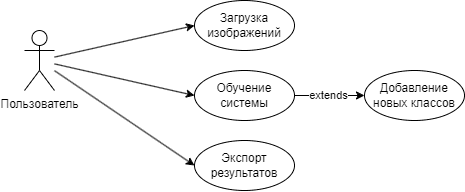
\includegraphics[width=0.8\linewidth]{usecase}
\caption{Диаграмма вариантов использования}
\label{usecase:image}
\end{figure}

На диаграмме представлены основные варианты использования приложения, включая загрузку изображений для распознавания, обучение системы, добавление новых классов объектов и экспорт результатов распознавания. Данная диаграмма помогает понять основные функциональные возможности приложения и взаимодействие с пользователями.

На основании анализа предметной области в программе должны быть реализованы следующие прецеденты:
\begin{enumerate}
\item Распознание объекта на изображении по его цветовым характеристикам;
\item Сохранение результатов распознания для дальнейшего использования;
\item Обучение и переобучение нейро-нечёткой сети;
\item Сохранение результатов обучения для дальнейшего расспознания.
\end{enumerate}

\subsection{Требования к оформлению документации}

Разработка программной документации и программного изделия должна производиться согласно ГОСТ 19.102-77 и ГОСТ 34.601-90. Единая система программной документации.

\section{Технический проект}
\subsection{Общая характеристика организации решения задачи}

Этот проект направлен на разработку системы, которая использует нечеткие нейронные сети для распознавания объектов на основе цветовых характеристик. Система будет способна анализировать изображения и выделять объекты, соответствующие заданным цветовым параметрам.

Основная цель - создание эффективной и точной системы распознавания объектов. Задачи включают:

\begin{itemize}
\item Разработка алгоритма нечеткой нейронной сети;
\item Создание базы данных для обучения и тестирования системы.
\end{itemize}

\subsection{Обоснование выбора технологии проектирования}

Нечеткие нейронные сети сочетают принципы нечеткой логики и нейронных сетей, что позволяет системе обрабатывать нечеткие и неточные данные, характерные для реальных изображений.

\subsubsection{Python и его библиотеки}

Python является предпочтительным языком программирования благодаря своей читаемости, простоте и обширной экосистеме библиотек, подходящих для работы с данными и машинным обучением:

\begin{itemize}
\item NumPy: Используется для эффективной работы с массивами и матрицами, что критично для обработки изображений и численных вычислений;
\item Pandas: Предоставляет удобные структуры данных для анализа и манипуляции данными;
\item Matplotlib/Seaborn: Библиотеки для визуализации данных, которые помогают в анализе результатов и представлении данных;
\item OpenCV: Открытая библиотека для работы с компьютерным зрением, которая может использоваться для предварительной обработки изображений;
\item TensorFlow/Keras: Популярные фреймворки для глубокого обучения, которые предоставляют инструменты для создания, обучения и тестирования нейронных сетей;
\item Scikit-learn: Библиотека для машинного обучения, предоставляющая различные алгоритмы классификации, регрессии и кластеризации.
\end{itemize}

\subsubsection{Архитектура нечёткой нейронной сети}

Архитектура нечёткой нейронной сети включает в себя 6 слоев с различными функциями:

Входной слой: Он содержит входные переменные, которые в данном случае представлены 3 цветовыми каналами изображения. Эти переменные обеспечивают начальную информацию для последующей обработки.

Два слоя фуззификации:

Второй слой: Ответственен за преобразование значений яркости изображения в степени принадлежности. Здесь присутствуют функции принадлежности для каждой переменной, их количество равно 3(Яркие, средние или тёмные оттенки цвета), что в совокупности создает 27 комбинаций. Эти функции помогают определить степень принадлежности значений.

Третий слой: На этом этапе для каждой переменной определяется функция принадлежности с наивысшим значением.

Слой базы нечётких правил: Четвертый слой содержит базу нечётких правил, которые добавляют веса функциям принадлежности. Эти правила используются для оценки значимости данных функций.

Слой дефуззификации: На этом этапе происходит обратное преобразование от степеней принадлежности к яркостным характеристикам.

Суммационный слой: Здесь происходит суммирование трех цветовых каналов для получения маски, которая может быть использована для выявления объектов на изображении. Эта маска может быть использована для поиска центров кластеров и других операций обработки данных.

\subsubsection{Описание базы данных}

База данных будет хранить информацию о различных моделях обучения нейронной сети. У каждой модели будет своя таблица, в которой будут храниться данные об одном наборе обучения нейронной сети и одной таблице с уже обученными значениями. Каждый набор обучения будет содержать четыре столбца: три столбца для входных значений, соответствующих трем цветовым каналам изображения, и один столбец для выходных значений.

ERD диаграмма структуры базы данных представлена на рисунке ~\ref{databasediagram:image}.

\begin{figure}[ht]
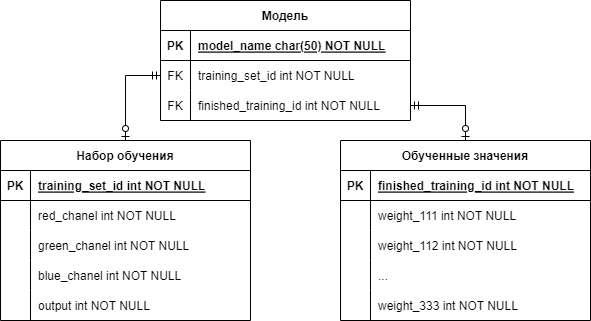
\includegraphics[width=1\linewidth]{databasediagram}
\caption{Диаграмма структуры базы данных}
\label{databasediagram:image}
\end{figure}

\subsection{Диаграмма компонентов}

Диаграмма компонентов представляет структуру системы в виде набора компонентов и их взаимосвязей. Каждый компонент отвечает за определенную функцию в рамках системы и может включать в себя подсистемы или модули.

\subsubsection{Структура компонентов}
На диаграмме компонентов изображены основные блоки системы, такие как:

\begin{itemize}
\item Графический интерфейс пользователя: Модуль, отвечающий за взаимодействие с пользователем, представление результатов и получение входных данных;
\item Модуль предварительной обработки данных: Отвечает за подготовку данных к анализу, включая фильтрацию шума и нормализацию изображений;
\item Модуль нечеткой нейронной сети: Ядро системы, реализующее алгоритмы обучения и распознавания объектов;
\item База данных: Хранит обучающий и тестовый наборы данных, а также результаты работы системы;
\item Модуль анализа данных: Производит анализ данных, классификацию и предоставляет статистику по результатам.
\end{itemize}

\subsubsection{Взаимодействие компонентов}
Компоненты системы взаимодействуют друг с другом следующим образом:

\begin{enumerate}
\item Пользователь загружает изображение через графический интерфейс пользователя;
\item Интерфейс передает изображение в модуль предварительной обработки данных;
\item После обработки данные передаются в модуль нечеткой нейронной сети для распознавания объектов;
\item Результаты распознавания сохраняются в базе данных;
\item Модуль анализа данных извлекает результаты из базы данных и представляет их пользователю через графический интерфейс пользователя.
\end{enumerate}

Диаграмма компонентов представленна на рисунке ~\ref{componentdiagram:image}.

\begin{figure}[ht]
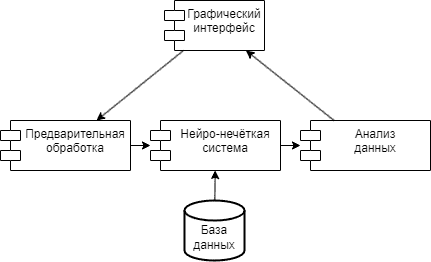
\includegraphics[width=1\linewidth]{componentdiagram}
\caption{Диаграмма компонентов системы}
\label{componentdiagram:image}
\end{figure}

\subsection{Содержание информационных блоков. Основные сущности}

Исходя из описания, можно выделить пять основных сущностей:

\begin{enumerate}
\item Графический интерфейс: Этот компонент отвечает за взаимодействие пользователя с нейронной сетью. Он представляет собой интерфейс, через который пользователь может отправлять данные на обработку, управлять обучающими данными нейронной сети и получать результаты;
\item Предварительная обработка: Эта сущность отвечает за предварительную обработку данных, поступающих от пользователя, чтобы подготовить их для дальнейшей работы нейронной сети. Здесь могут проводиться различные операции, такие как нормализация данных, фильтрация шума и преобразование формата;
\item Нейронная сеть: В данном участке происходит распознавание объектов на обработанном изображении с использованием выбранной модели или проведение обучения новой модели на выбранном наборе обучающих данных;
\item База данных: В этой части системы хранится информация о наборах обучающих данных и обученных моделях нейронной сети. База данных предоставляет доступ к данным для обучения и позволяет сохранять результаты работы нейронной сети для последующего использования;
\item Анализ данных: Этот компонент отвечает за анализ данных, полученных из нейронной сети. Здесь могут проводиться различные вычисления и визуализация результатов работы нейронной сети, а также их сохранение и представление пользователю.
\end{enumerate}

\subsubsection{Структура сущности графический интерфейс}
Графический интерфейс хранит в себе методы:

\begin{enumerate}
\item Запрос файла изображения у пользователя;
\item Выбор нужного набра обучения, для обучения нейроной сети;
\item Выбор нужной модели для расспознания объектов;
\item Запуск обучения, который вызовет метод обучения из сущности нейронной сети;
\item Запуск распознания, который вызовет метод обработки из сущности предварительной обработки;
\item Запрос методов анализа данных, полученных из нейронной сети из сущности анализа данных.
\end{enumerate}

\subsubsection{Структура сущности предварительная обработка}
Предварительная обработка осуществляет преобразование входящего изображения в формат, необходимый для работы нейронной сети.

\subsubsection{Структура сущности нейронная сеть}
Нейронная сеть строится в соответствии со структурой, описанной выше, и включает в себя два основных метода: обучение и распознавание объектов.

\subsubsection{Структура сущности база данных}
База данных предоставляет информацию для обучения и распознавания объектов нейронной сети, а также для сохранения новых обученных моделей.

\subsubsection{Структура сущности анализ данных}
Анализ данных включает в себя различные методы преобразования полученных от нейронной сети значений в полезные данные, такие как центры кластеров, количественное содержание цветов на изображении и другие.
\ifПрактика{}\else{
   \section{Рабочий проект}
\subsection{Классы, используемые при разработке сайта}

Список классов и методов, которые были использованы при создании приложения представлены на таблице \ref{class:table}.

\renewcommand{\arraystretch}{0.8} % уменьшение расстояний до сетки таблицы
\begin{xltabular}{\textwidth}{|X|p{2.5cm}|>{\setlength{\baselineskip}{0.7\baselineskip}}p{4.85cm}|>{\setlength{\baselineskip}{0.7\baselineskip}}p{4.85cm}|}
\caption{Описание классов, используемых в приложении\label{class:table}}\\
\hline \centrow \setlength{\baselineskip}{0.7\baselineskip} Название класса & \centrow \setlength{\baselineskip}{0.7\baselineskip} Модуль, к которому относится класс & \centrow Описание класса & \centrow Методы \\
\hline \centrow 1 & \centrow 2 & \centrow 3 & \centrow 4\\ \hline
\endfirsthead
\caption*{Продолжение таблицы \ref{class:table}}\\
\hline \centrow 1 & \centrow 2 & \centrow 3 & \centrow 4\\ \hline
\finishhead
ANFIS & Нейронная сеть & ANFIS – класс, в котором осуществляется идентификация объектов с использованием нечеткой нейросети. & нормализацияКаналов( ПутьФайла)

Происходит загрузка изображения из файла, последующее его разделение на цветовые каналы, а затем преобразование этих каналов, представленных в виде матриц, в массивы. После этого происходит нормализация значений яркости.

АнфисаРаспознать( Путь, ИмяМодели)

В рамках данной функции осуществляется прием данных, обработанных методом нормализацияКаналов.\\
\hline & & & Эти данные, совмещенные с оптимизированной моделью искусственной нейронной сети, подвергаются дальнейшей обработке в модуле anfisReady, который разработан на основе программного обеспечения MATLAB. Завершающим этапом является генерация черно-белой маски, которая визуализирует распознанные объекты и имеет разрешение 720x720 пикселей

АнфисаТренировать( Набор, Размер, ИмяМодели)

Инициируя процесс обучения, функция использует предоставленный набор данных и его объем для конфигурации модуля anfis, реализованного в среде MATLAB. На основании этих данных функция строит и оптимизирует модель нечеткой нейронной сети. После успешного обучения, сформированная модель сохраняется в базу данных с наименованием, указанным в параметрах функции.\\
\hline & & & function out = AnfisReady(data, name)
 
Данная функция, реализованная на языке программирования MATLAB и использующая среду выполнения MATLAB Runtime, осуществляет передачу данных в нейронную сеть на пиксельном уровне. В соответствии с выбранной моделью нейросети, функция вычисляет степень соответствия каждого пикселя заданной модели и возвращает количественную оценку этого соответствия.

function out = Anfis(data, name)

Программный модуль, реализованный на языке программирования MATLAB и эксплуатирующий среду выполнения MATLAB Runtime, предназначен для приема набора данных, представляющих собой тренировочную выборку. Данный модуль осуществляет процесс обучения нечеткой нейронной сети, используя предоставленные данные.\\
\hline & & & В результате выполнения, модуль выдает модель нечеткой нейронной сети, прошедшую процедуру обучения.\\
\hline DB & База данных & DB – Класс для работы с базой данных & сохранить(ИмяМодели, Набор)

Данная функция реализует процедуру архивации тренировочного датасета и соответствующей обученной нейросетевой модели в структурированное хранилище данных. Это обеспечивает сохранность исходных обучающих данных и параметров модели для последующего использования и анализа.

загрузитьСписокНаборов()

Функциональный модуль предназначен для извлечения данных из базы данных, содержащей информацию о тренировочных наборах и соответствующих обученных нейронных моделях.\\
\hline & & & Он выполняет операцию чтения и последующего формирования перечня доступных тренировочных наборов данных и ассоциированных с ними моделей.

загрузитьНабор(Название)

Эта функция осуществляет операцию извлечения из базы данных специфического обучающего набора, состоящего из трёх цветовых каналов и целевого значения.\\
\hline main & Графический интерфейс & main – Класс для взаимодействия с пользователем & загрузитьИзображение()

Данная функция выполняет загрузку изображения из файла, а затем проводит его масштабирование до определённых размеров 720x720 пикселей, что обеспечивает его корректное отображение в заданном графическом интерфейсе пользователя.\\
\hline & & & 

распознать()

Функция инициирует процесс передачи ранее загруженного изображения в архитектуру нейронной сети, после чего активирует интерфейс для выбора предварительно обученной модели из доступных вариантов, что позволяет пользователю взаимодействовать с системой машинного обучения.

выбрать(ОкноВыбора)

Данная функция осуществляет интеграцию предварительно обученной модели в структуру нейронной сети, после чего производит деактивацию интерфейса выбора.

сохранитьРезультатРаспознания()

Функция инициирует активацию диалогового интерфейса, предназначенного для сохранения выходных данных нейронной сети в файловую систему, обеспечивая тем самым персистентность результатов вычислений.\\
\hline & & & 

обучать()

Функция активирует пользовательский интерфейс в виде диалогового окна, которое предоставляет возможность выбора набора данных для обучения нейронной сети.

подтвердить(ОкноВыбора)

Функция инициирует передачу выбранного или вновь созданного датасета для обучения нейронной сети, после чего активируется интерфейс в виде диалогового окна, предоставляющего пользователю опцию присвоения наименования новой модели.

отправить(ОкноНазвания)

Эта функция осуществляет трансмиссию наименования модели в архитектуру нейронной сети, инициируя этим процедуру обучения.\\
\hline & & & По завершении процесса, модель систематически регистрируется и архивируется в соответствующей базе данных, что обеспечивает её доступность для дальнейшего использования и интеграции в различные прикладные задачи машинного обучения.
\end{xltabular}
\renewcommand{\arraystretch}{1.0} % восстановление сетки

\subsection{Модульное тестирование разработанного приложения}

Модульные тесты для класса ANFIS из модели данных представлены на рисунках \ref{test1:image}-\ref{test3:image}.

\begin{figure}[ht]
\begin{lstlisting}[language=Python]
import os
import unittest
from PIL import Image
import anfis
import numpy as np
import matlab
from random import shuffle
from ANFIS import нормализацияКаналов
from ANFIS import АнфисаРаспознать

class TestНормализацияКаналов(unittest.TestCase):
    def test_нормализация_существующего_файла(self):
        результат = нормализацияКаналов('test_image.png')
        self.assertIsNotNone(результат, "Функция должна возвращать не None для существующего файла")
        self.assertTrue((результат >= 0).all() and (результат <= 1).all(), "Все значения должны быть в диапазоне от 0 до 1")
    def test_нормализация_несуществующего_файла(self):
        результат = нормализацияКаналов('несуществующий_файл.jpg')
        self.assertIsNone(результат, "Функция должна возвращать None для несуществующего файла")
\end{lstlisting}  
\caption{Модульный тест метода нормализацияКаналов класса ANFIS}
\label{test1:image}
\end{figure}

\begin{figure}[ht]
\begin{lstlisting}[language=Python]
import os
import unittest
from PIL import Image
import anfis
import numpy as np
import matlab
from random import shuffle
from ANFIS import нормализацияКаналов
from ANFIS import АнфисаРаспознать

class TestАнфисаРаспознать(unittest.TestCase):
    def setUp(self):
        self.путь = 'test_image.png'
        self.имяМодели = 'test_model_name'
    def test_распознавание_изображения(self):
        результат = АнфисаРаспознать(self.путь, self.имяМодели)
        self.assertIsInstance(результат, Image.Image, "Функция должна возвращать объект изображения")
    def test_сохранение_изображения(self):
        результат = АнфисаРаспознать(self.путь, self.имяМодели)
        self.assertTrue(os.path.isfile('output_image.png'), "Файл изображения должен быть сохранён")
\end{lstlisting}  
\caption{Модульный тест метода АнфисаРаспознать класса ANFIS}
\label{test2:image}
\end{figure}

\begin{figure}[ht]
\begin{lstlisting}[language=Python]
import os
import unittest
from PIL import Image
import anfis
import numpy as np
import matlab
from random import shuffle
from ANFIS import нормализацияКаналов
from ANFIS import АнфисаРаспознать

class TestНормализацияКаналов(unittest.TestCase):
    def test_нормализация_существующего_файла(self):
        результат = нормализацияКаналов('test_image.png')
        self.assertIsNotNone(результат, "Функция должна возвращать не None для существующего файла")
        self.assertTrue((результат >= 0).all() and (результат <= 1).all(), "Все значения должны быть в диапазоне от 0 до 1")
    def test_нормализация_несуществующего_файла(self):
        результат = нормализацияКаналов('несуществующий_файл.jpg')
        self.assertIsNone(результат, "Функция должна возвращать None для несуществующего файла")
\end{lstlisting}  
\caption{Модульный тест метода нормализацияКаналов класса ANFIS}
\label{test3:image}
\end{figure}

Модульные тесты для класса DB из модели данных представлены на рисунках \ref{test4:image}-\ref{test6:image}.

\begin{figure}[ht]
\begin{lstlisting}[language=Python]
from DB import сохранить
from DB import загрузитьСписокНаборов
from DB import загрузитьНабор

class TestСохранить(unittest.TestCase):
    def setUp(self):
        self.ИмяМодели = 'test_model'
        self.Набор = [(1, 2, 3, 4), (5, 6, 7, 8)]
        self.Подключение = sqlite3.connect(':memory:')
        self.Курсор = self.Подключение.cursor()
        self.Курсор.execute('''CREATE TABLE Готовые_данные (Адрес_файла TEXT)''')
        self.Курсор.execute('''CREATE TABLE Тренировочный_набор (Красный_канал INTEGER, Синий_канал INTEGER, Зелёный_канал INTEGER, Выходные_данные INTEGER)''')
        self.Курсор.execute('''CREATE TABLE Модель (Имя_модели TEXT, ИД_Тренировочного_набора INTEGER, ИД_Готовых_данных INTEGER)''')
    def test_подключение_к_базе(self):
        self.assertIsNotNone(self.Подключение, "Должно быть установлено подключение к базе данных")
    def test_добавление_в_готовые_данные(self):
        сохранить(self.ИмяМодели, self.Набор)
        self.Курсор.execute("SELECT * FROM Готовые_данные WHERE Адрес_файла = ?", (self.ИмяМодели,))
        результат = self.Курсор.fetchone()
        self.assertIsNotNone(результат, "Модель должна быть добавлена в таблицу Готовые_данные")
    def test_добавление_в_тренировочный_набор(self):
        сохранить(self.ИмяМодели, self.Набор)
        for данные in self.Набор:
            self.Курсор.execute("SELECT * FROM Тренировочный_набор WHERE Красный_канал = ? AND Синий_канал = ? AND Зелёный_канал = ? AND Выходные_данные= ?", данные)
            результат = self.Курсор.fetchone()
            self.assertIsNotNone(результат, "Данные должны быть добавлены в таблицу Тренировочный_набор")
    def test_закрытие_подключения(self):
        self.Подключение.close()
        self.assertRaises(sqlite3.ProgrammingError, self.Курсор.execute, "SELECT * FROM Готовые_данные")
    def tearDown(self):
        self.Подключение.close()
\end{lstlisting}  
\caption{Модульный тест метода загрузитьНабор класса DB}
\label{test4:image}
\end{figure}

\begin{figure}[H]
\begin{lstlisting}[language=Python]
from DB import сохранить
from DB import загрузитьСписокНаборов
from DB import загрузитьНабор

class TestЗагрузитьСписокНаборов(unittest.TestCase):
    def setUp(self):
        self.Подключение = sqlite3.connect(':memory:')
        self.Курсор = self.Подключение.cursor()
        self.Курсор.execute('''CREATE TABLE Готовые_данные (Адрес_файла TEXT)''')
        self.Курсор.executemany("INSERT INTO Готовые_данные (Адрес_файла) VALUES (?)", [('file1',), ('file2',), ('file3',)])

    def test_загрузка_списка(self):
        ожидаемый_список = ['file1', 'file2', 'file3']
        результат = загрузитьСписокНаборов()
        self.assertEqual(результат, ожидаемый_список, "Список наборов должен соответствовать ожидаемому")

    def test_закрытие_подключения(self):
        загрузитьСписокНаборов()
        self.assertRaises(sqlite3.ProgrammingError, self.Курсор.execute, "SELECT * FROM Готовые_данные")

    def tearDown(self):
        self.Подключение.close()
\end{lstlisting}  
\caption{Модульный тест метода загрузитьСписокНаборов класса DB}
\label{test5:image}
\end{figure}

\begin{figure}[H]
\begin{lstlisting}[language=Python]
from DB import сохранить
from DB import загрузитьСписокНаборов
from DB import загрузитьНабор

class TestЗагрузитьНабор(unittest.TestCase):
    def setUp(self):
        Название = 'test_model'
        self.Подключение = sqlite3.connect(':memory:')
        self.Курсор = self.Подключение.cursor()
        self.Курсор.execute('''CREATE TABLE Модель (Имя_модели TEXT, ИД_Тренировочного_набора INTEGER)''')
        self.Курсор.execute('''CREATE TABLE Тренировочный_набор (ИД_тренировочного_набора INTEGER, Красный_канал INTEGER, Синий_канал INTEGER, Зелёный_канал INTEGER, Выходные_данные INTEGER)''')
        self.Курсор.execute("INSERT INTO Модель (Имя_модели, ИД_Тренировочного_набора) VALUES (?, ?)", (Название, 1))
        self.Курсор.execute("INSERT INTO Тренировочный_набор (ИД_тренировочного_набора, Красный_канал, Синий_канал, Зелёный_канал, Выходные_данные) VALUES (1, 255, 0, 0, 1)")

    def test_загрузка_набора(self):
        ожидаемый_выход = [(255, 0, 0, 1)]
        результат = загрузитьНабор('test_model')
        self.assertEqual(результат[0], ожидаемый_выход, "Загруженный набор должен соответствовать ожидаемому")

    def test_формат_выходных_данных(self):
        результат = загрузитьНабор('test_model')
        self.assertEqual(результат[1], (1, 4), "Формат выходных данных должен быть кортежем с размерностью набора")

    def test_закрытие_подключения(self):
        загрузитьНабор('test_model')
        self.assertRaises(sqlite3.ProgrammingError, self.Курсор.execute, "SELECT * FROM Модель")

    def tearDown(self):
        self.Подключение.close()
\end{lstlisting}  
\caption{Модульный тест метода загрузитьНабор класса DB}
\label{test6:image}
\end{figure}
\subsection{Системное тестирование разработанного приложения}

На рисунке \ref{systemtest_interface:image} представлен интерфейс программы.
\begin{figure}[H]
\centering
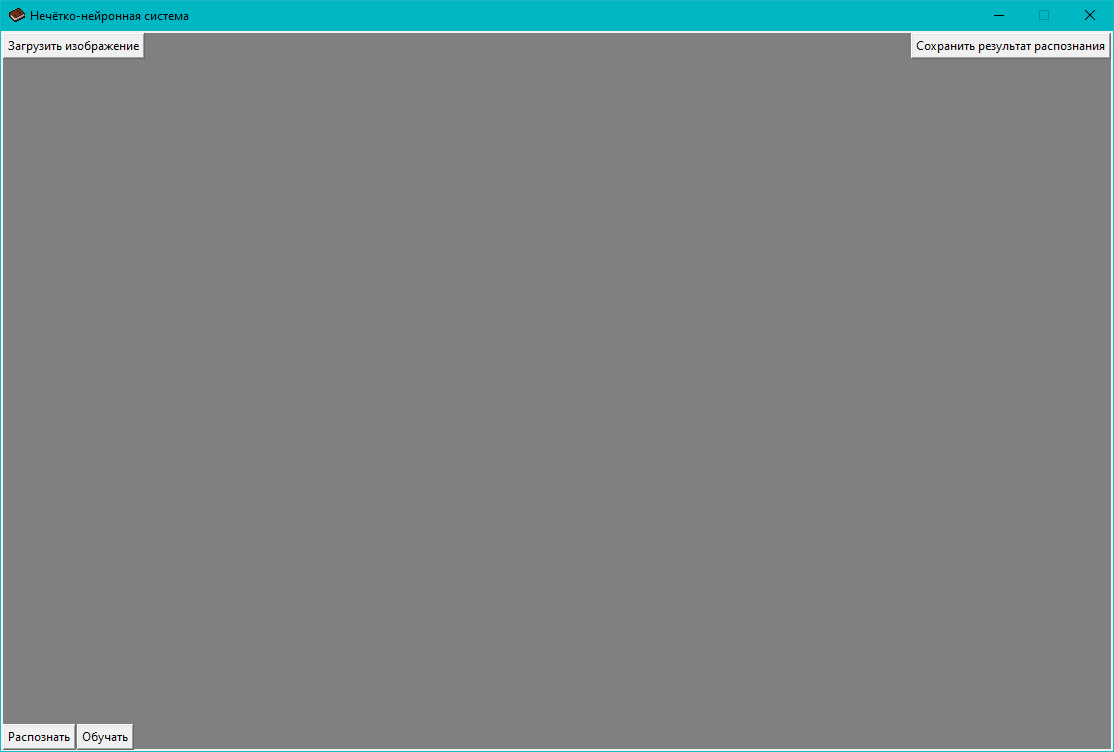
\includegraphics[width=1\linewidth]{systemtest_interface}
\caption{Диаграмма вариантов использования}
\label{systemtest_interface:image}
\end{figure}

На рисунках \ref{systemtest_responce:image}-\ref{systemtest_responce4:image} представлен полный путь распознания объекта на изображении.

\begin{figure}[H]
\center{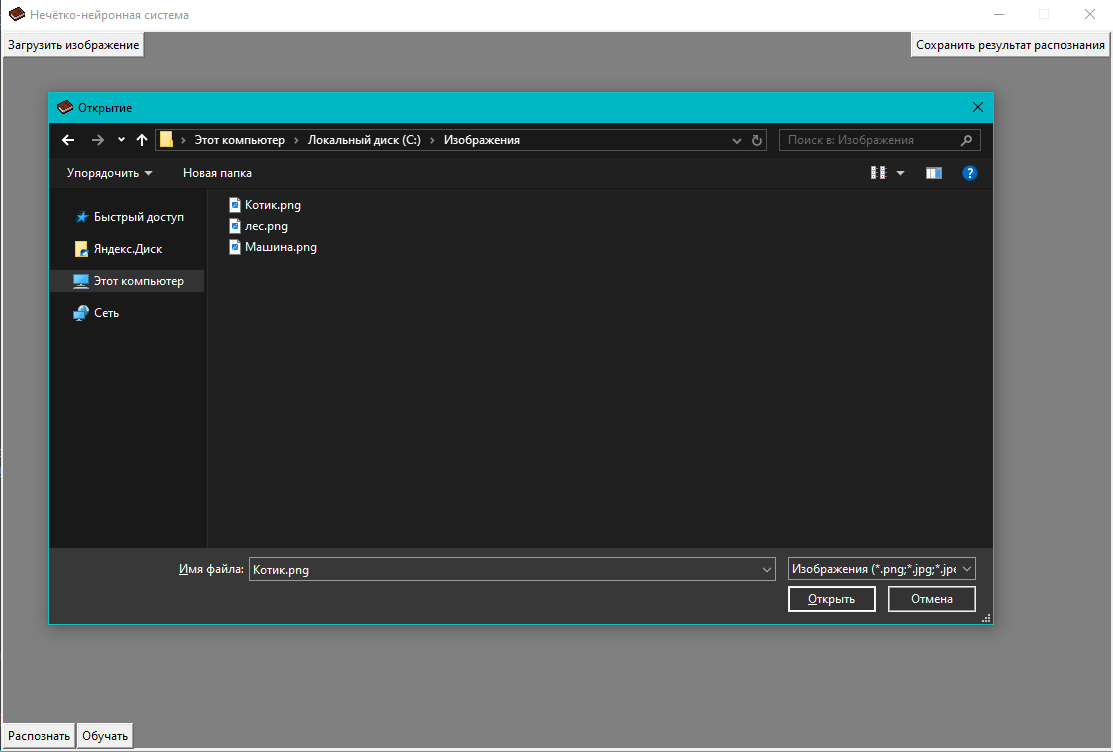
\includegraphics[width=1\linewidth]{systemtest_responce}}
\caption{Диалоговое окно загрузки файла Машина.png}
\label{systemtest_responce:image}
\end{figure}

\begin{figure}[H]
\center{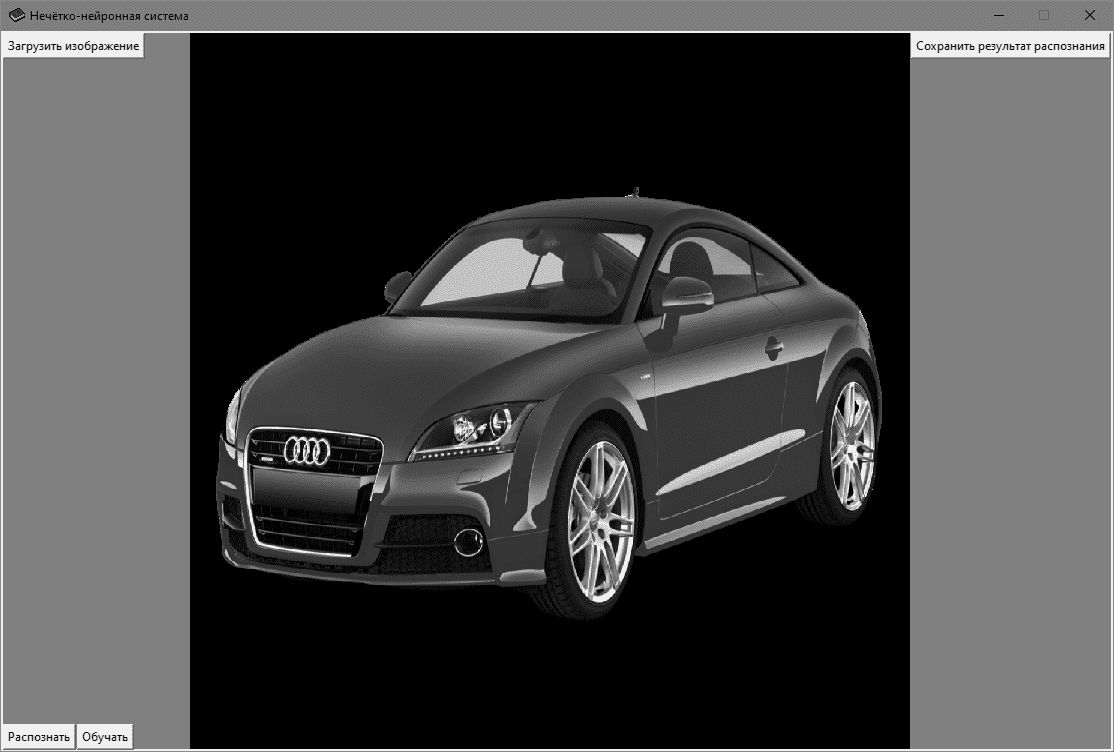
\includegraphics[width=1\linewidth]{systemtest_responce1}}
\caption{Изображение отображено в интерфейсе программы}
\label{systemtest_responce1:image}
\end{figure}

\begin{figure}[H]
\center{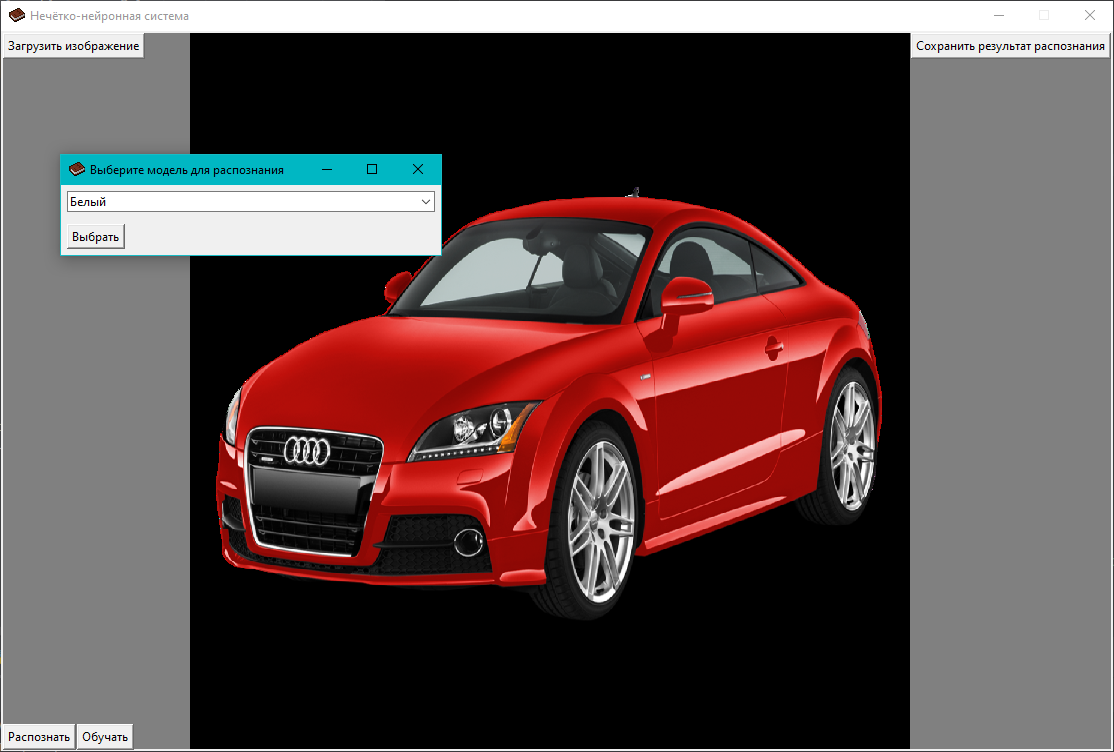
\includegraphics[width=1\linewidth]{systemtest_responce2}}
\caption{Окно выбора модели для распознания}
\label{systemtest_responce2:image}
\end{figure}

\begin{figure}[H]
\center{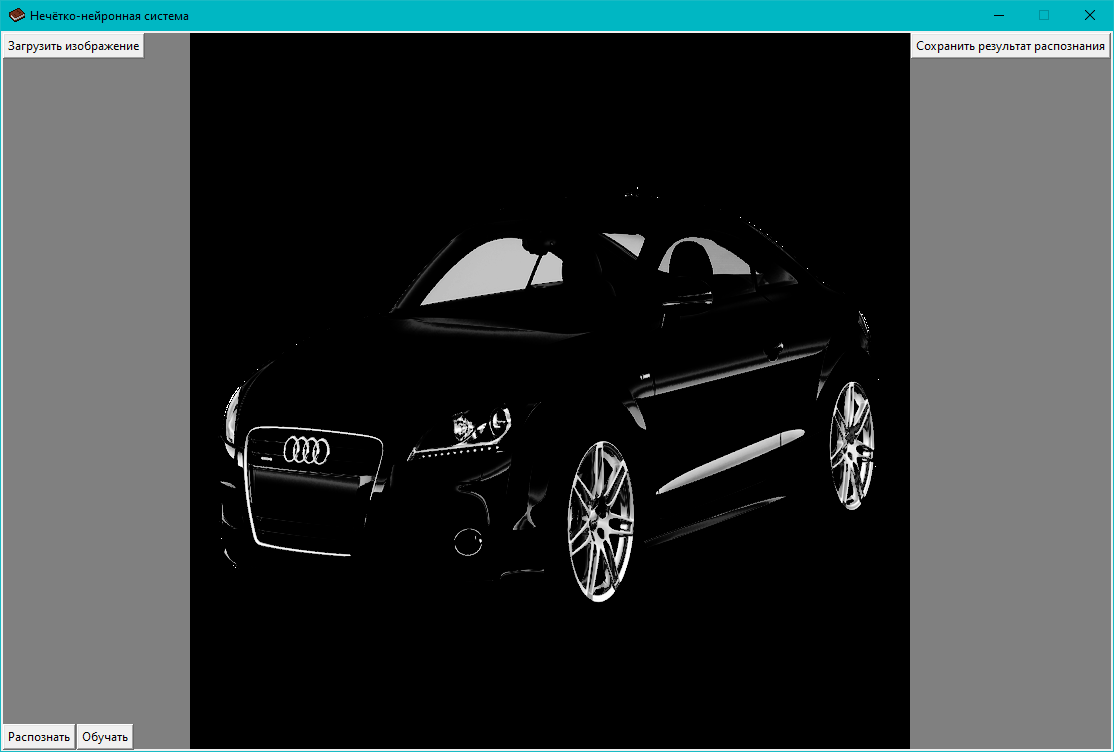
\includegraphics[width=1\linewidth]{systemtest_responce3}}
\caption{Распознанный объект отображен на интерфейсе}
\label{systemtest_responce3:image}
\end{figure}

\begin{figure}[H]
\center{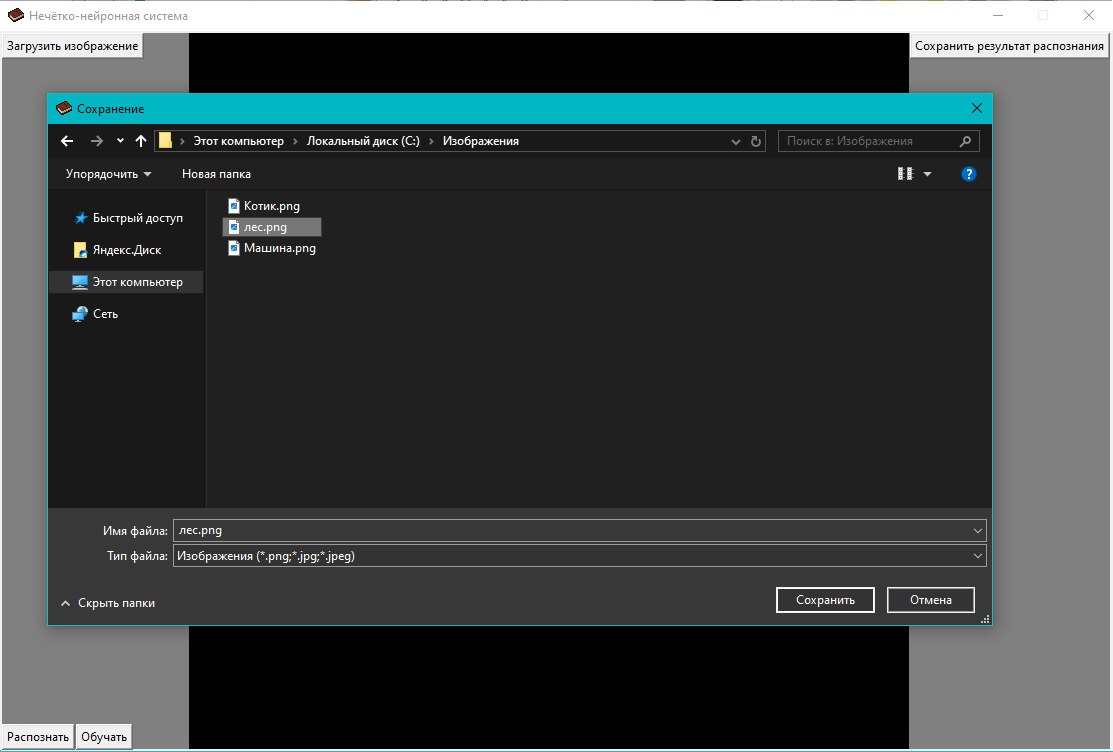
\includegraphics[width=1\linewidth]{systemtest_responce4}}
\caption{Диалоговое окно сохранения результата}
\label{systemtest_responce4:image}
\end{figure}

На рисунках \ref{systemtest_train1:image}-\ref{systemtest_train3:image} представлены все варианты обучения нейронной сети.

На рисунке \ref{systemtest_train1:image} была нажата кнопка обучать, после чего открылось окно выбора набора.

\begin{figure}[H]
\center{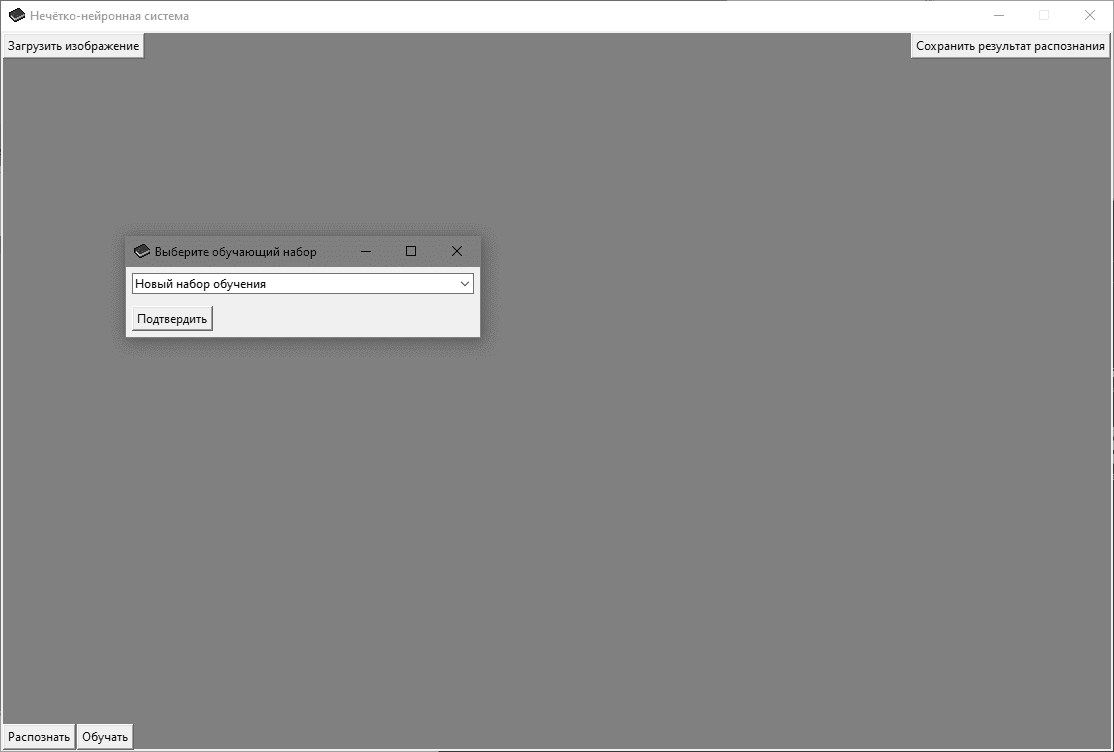
\includegraphics[width=1\linewidth]{systemtest_train1}}
\caption{Окно выбора обучающего набора}
\label{systemtest_train1:image}
\end{figure}

После выбора нового набора появилось окно, предлагающее назвать модель и обучить её.

\begin{figure}[H]
\center{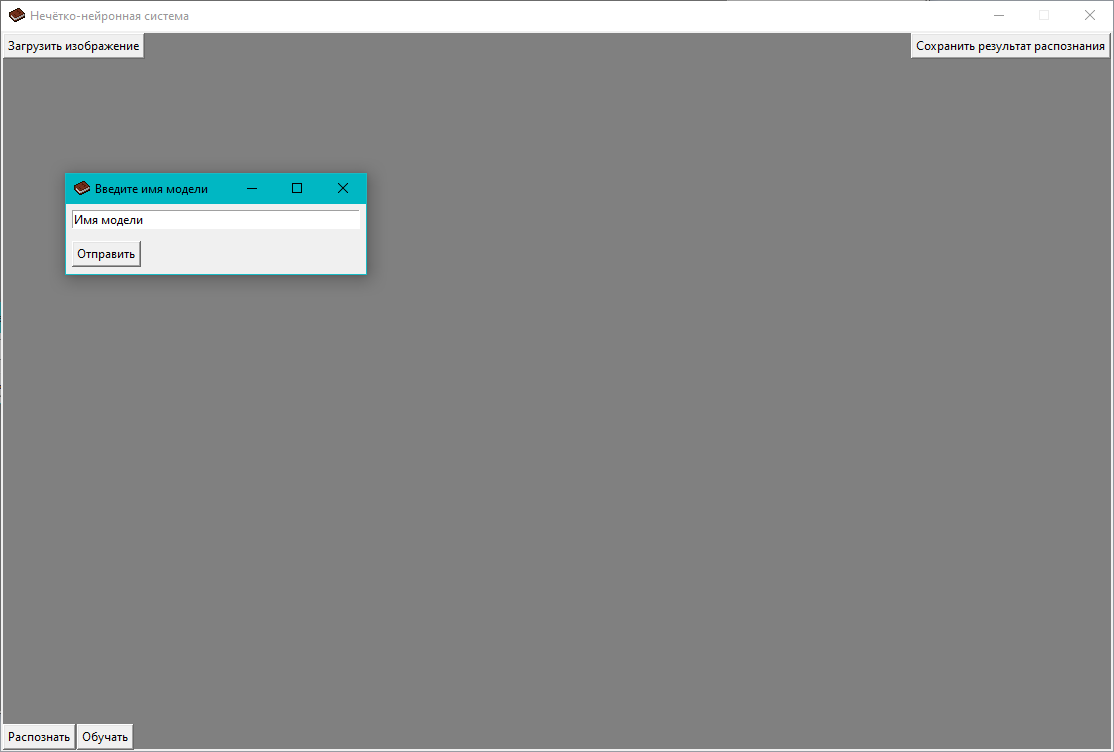
\includegraphics[width=1\linewidth]{systemtest_train2}}
\caption{Окно выбора названия новой модели}
\label{systemtest_train2:image}
\end{figure}

Вместо создания нового набора, после нажатия кнопки обучать, можно выбрать заготовленный набор и обучить нейронную сеть по нему.

\begin{figure}[H]
\center{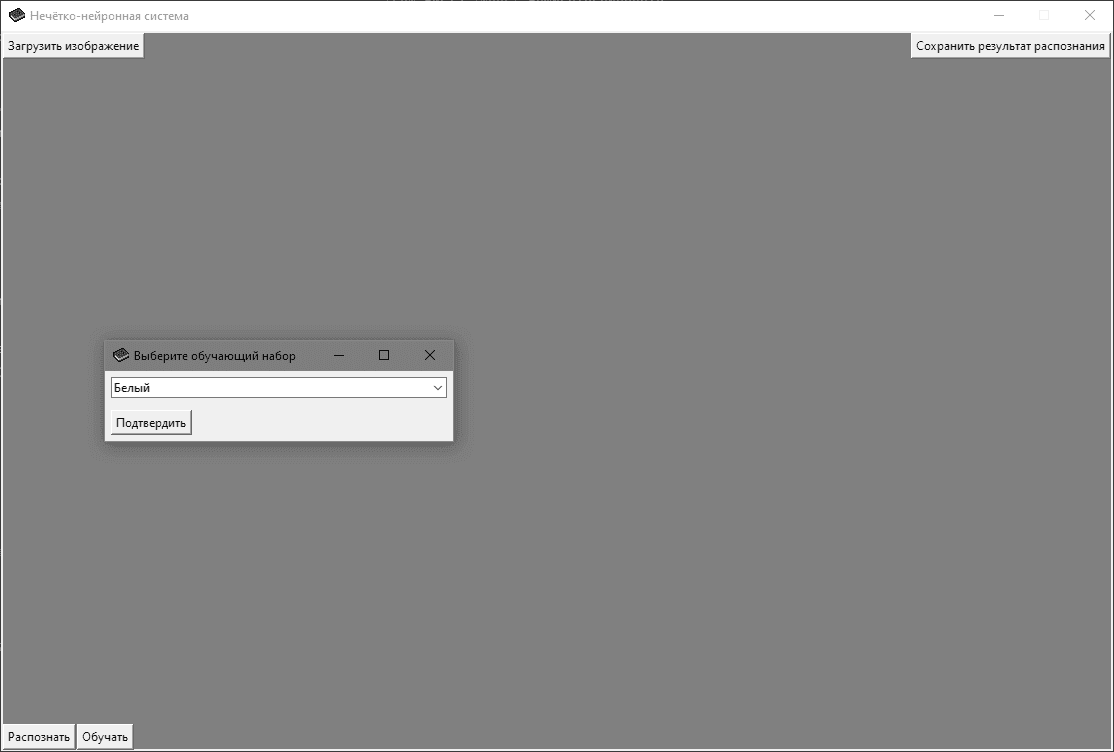
\includegraphics[width=1\linewidth]{systemtest_train3}}
\caption{Выбор обучения по набору ''Белый''}
\label{systemtest_train3:image}
\end{figure}

На рисунке \ref{systemtest_responce5:image} было загружено изображение кошки.

\begin{figure}[H]
\center{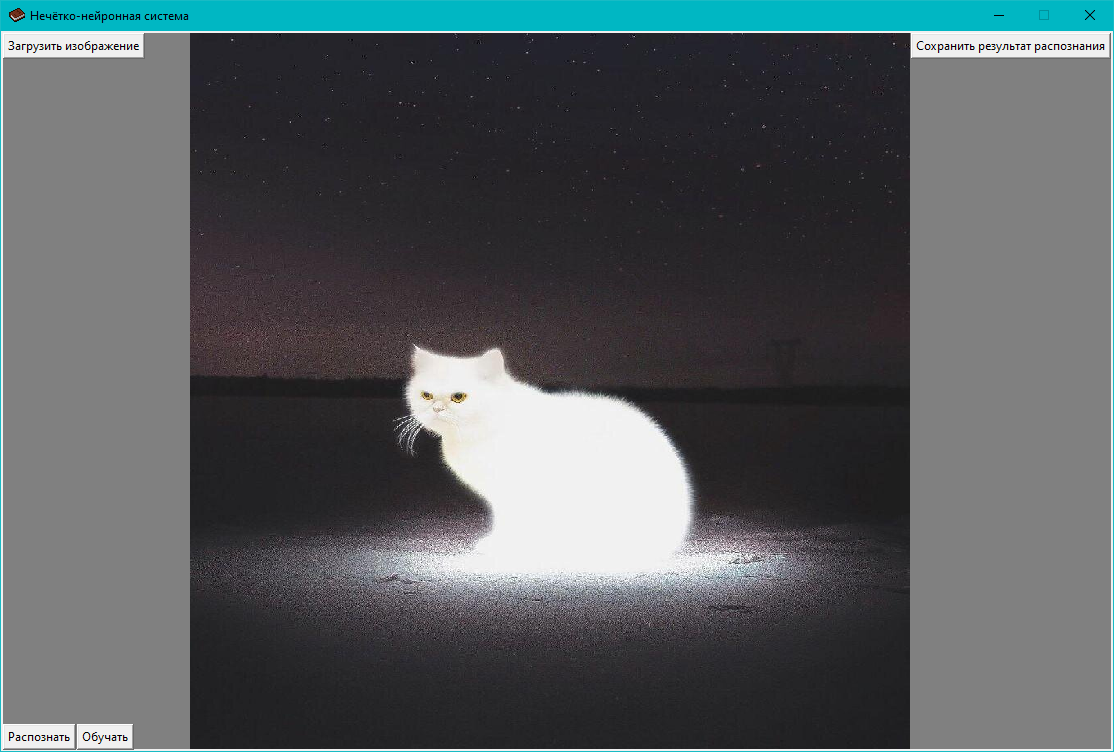
\includegraphics[width=1\linewidth]{systemtest_responce5}}
\caption{Интерфейс с изображением кошки}
\label{systemtest_responce5:image}
\end{figure}

На рисунке \ref{systemtest_responce6:image} изображение кошки было обработано по модели ''Белый''.

\begin{figure}[H]
\center{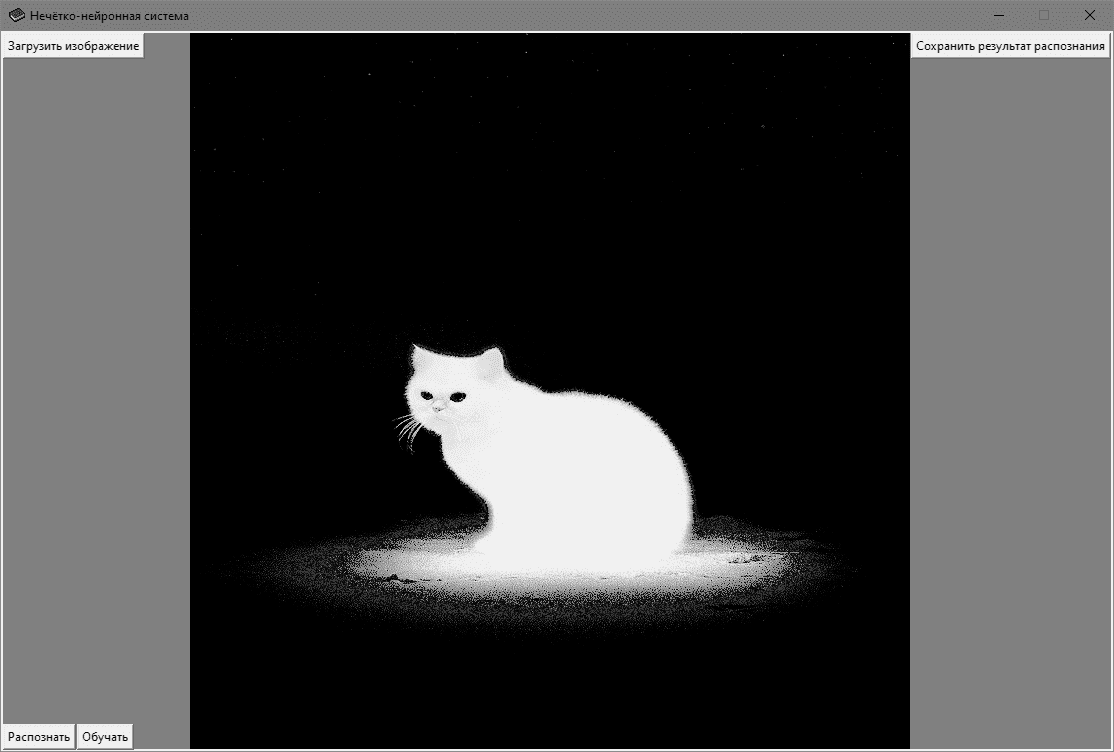
\includegraphics[width=1\linewidth]{systemtest_responce6}}
\caption{Распознанныйе объекты на изображении кошки}
\label{systemtest_responce6:image}
\end{figure}
На рисунке \ref{systemtest_responce7:image} было загружено изображение лилии.

\begin{figure}[H]
\center{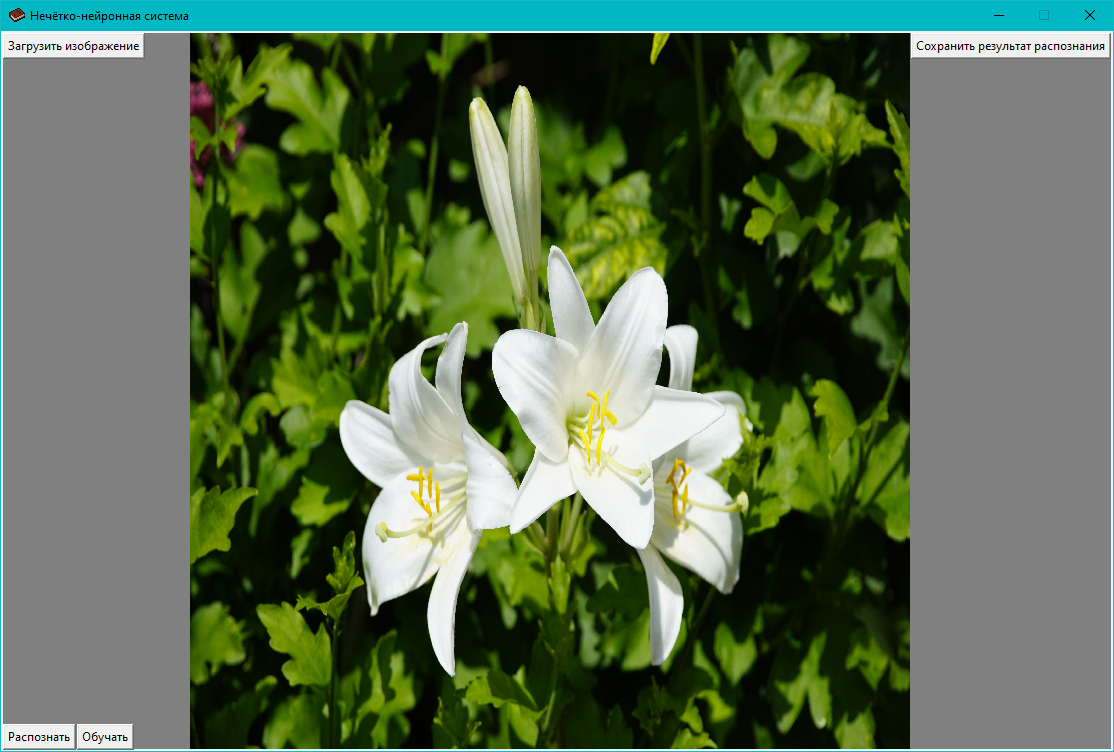
\includegraphics[width=1\linewidth]{systemtest_responce7}}
\caption{Интерфейс с изображением лилии}
\label{systemtest_responce7:image}
\end{figure}

На рисунке \ref{systemtest_responce8:image} изображение лилии было обработано по модели ''Белый''.

\begin{figure}[H]
\center{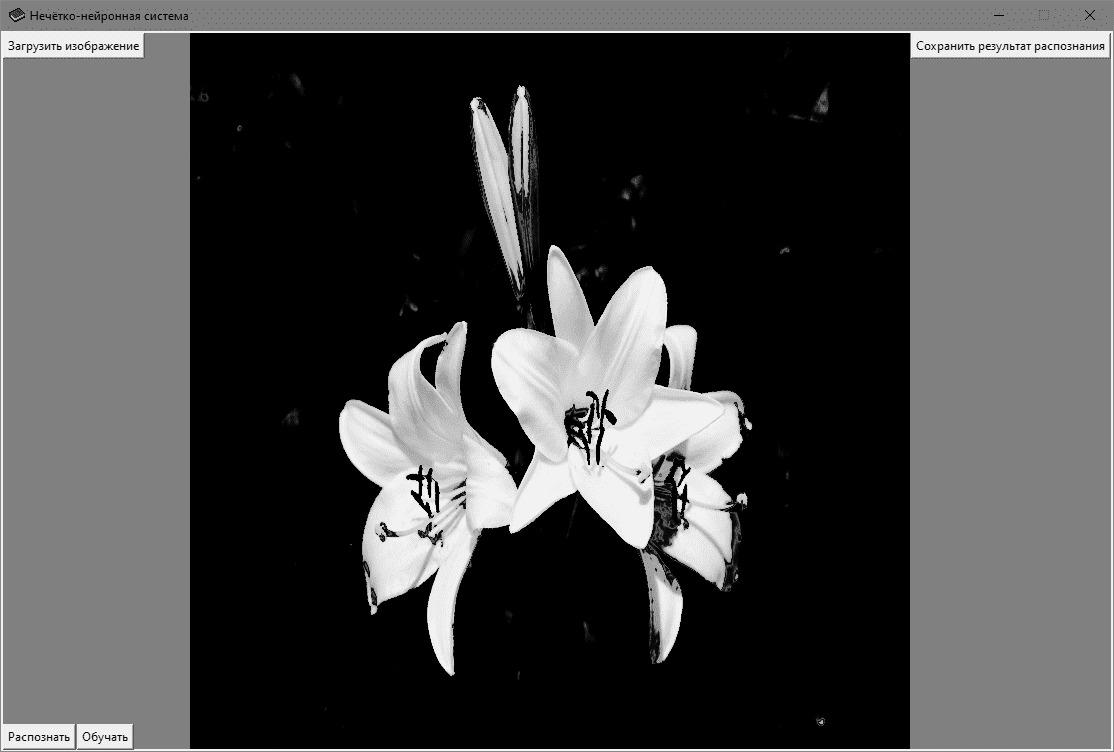
\includegraphics[width=1\linewidth]{systemtest_responce8}}
\caption{Распознанныйе объекты на изображении лилии}
\label{systemtest_responce8:image}
\end{figure}
На рисунке \ref{systemtest_responce9:image} было загружено изображение леса.

\begin{figure}[H]
\center{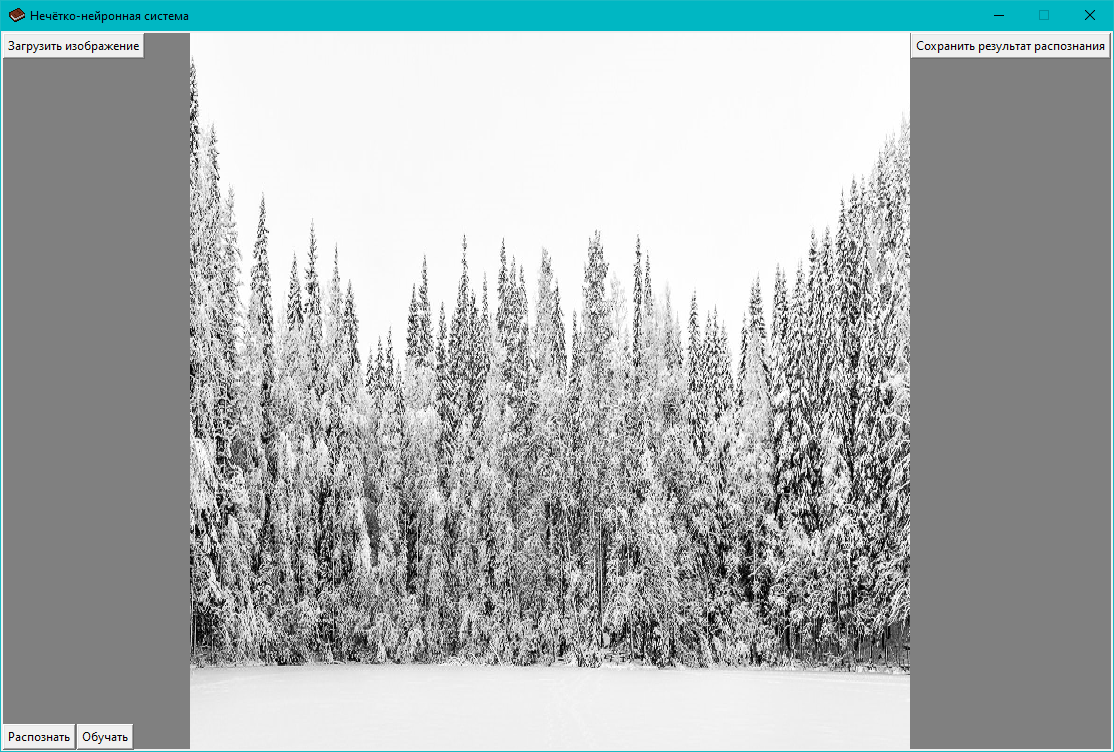
\includegraphics[width=1\linewidth]{systemtest_responce9}}
\caption{Интерфейс с изображением леса}
\label{systemtest_responce9:image}
\end{figure}

На рисунке \ref{systemtest_responce10:image} изображение леса было обработано по модели ''Белый''.

\begin{figure}[H]
\center{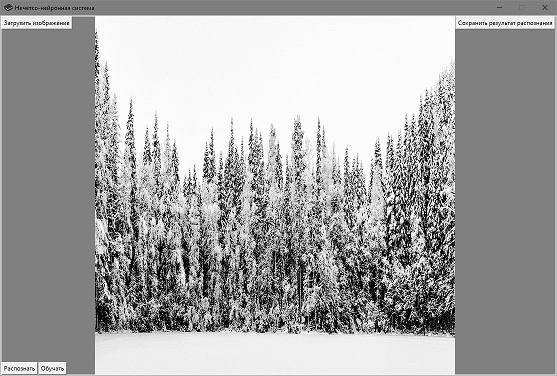
\includegraphics[width=1\linewidth]{systemtest_responce10}}
\caption{Распознанныйе объекты на изображении леса}
\label{systemtest_responce10:image}
\end{figure}
На рисунке \ref{systemtest_responce11:image} было загружено изображение футбола.

\begin{figure}[H]
\center{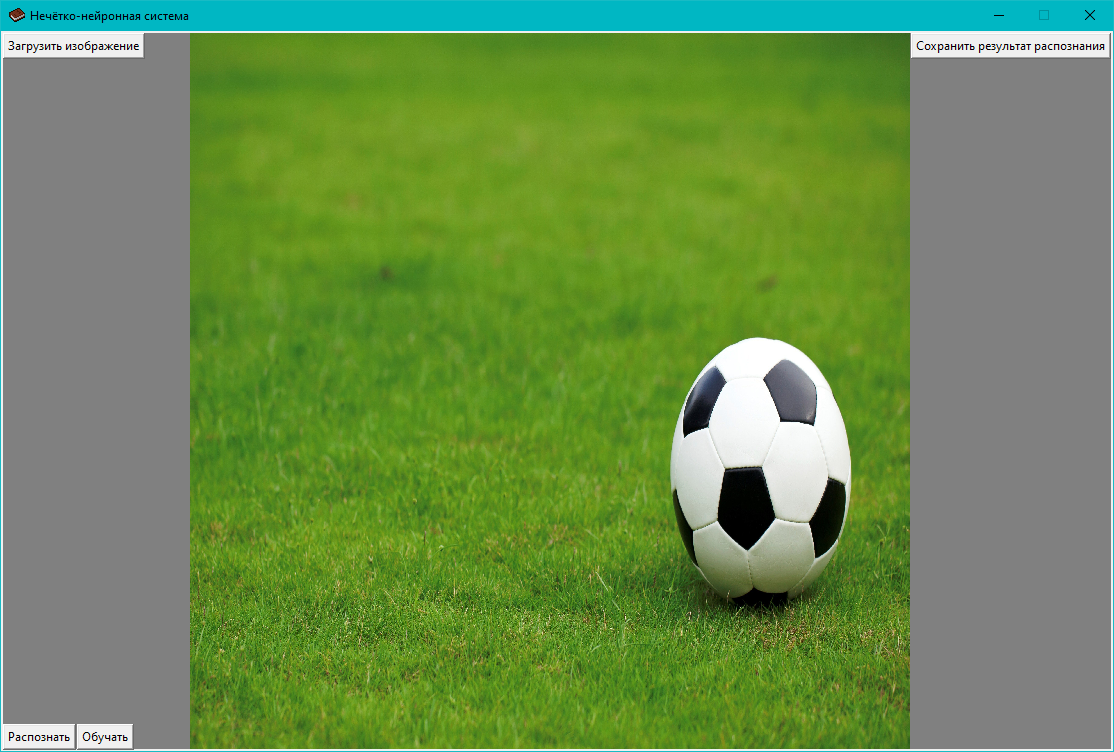
\includegraphics[width=1\linewidth]{systemtest_responce11}}
\caption{Интерфейс с изображением футбола}
\label{systemtest_responce11:image}
\end{figure}

На рисунке \ref{systemtest_responce12:image} изображение футбола было обработано по модели ''Белый''.

\begin{figure}[H]
\center{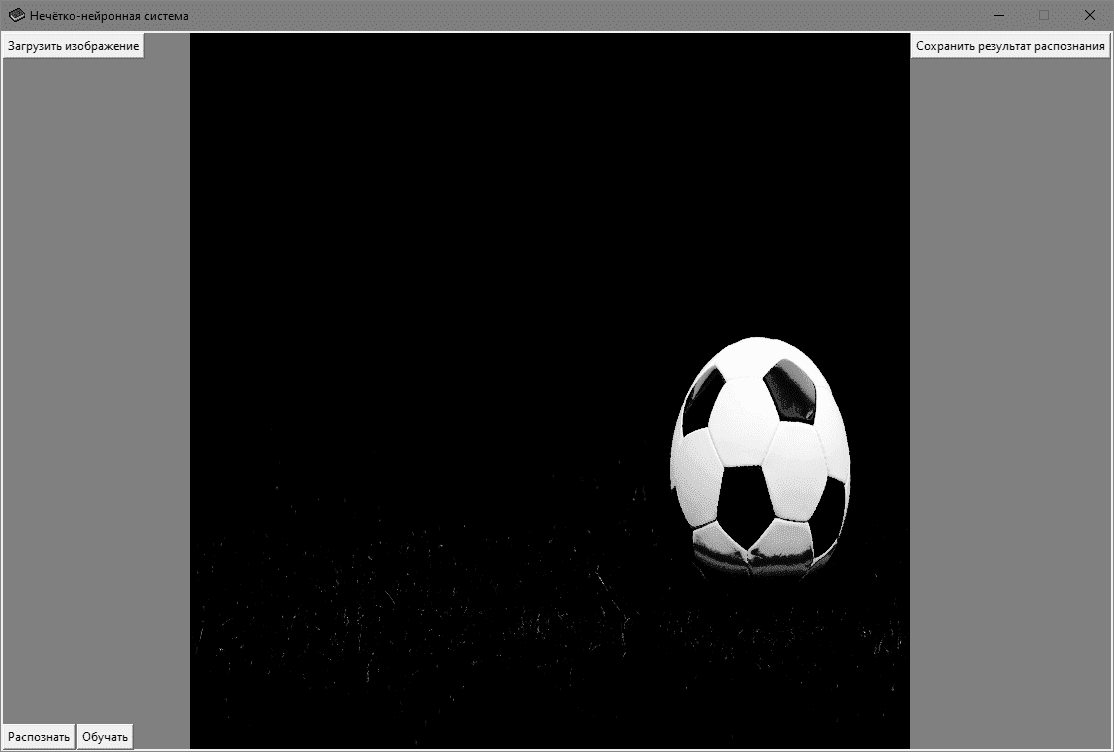
\includegraphics[width=1\linewidth]{systemtest_responce12}}
\caption{Распознанныйе объекты на изображении футбола}
\label{systemtest_responce12:image}
\end{figure}
На рисунке \ref{systemtest_responce13:image} было загружено изображение платья.

\begin{figure}[H]
\center{
\includegraphics[width=1\linewidth]{systemtest_responce13}}
\caption{Интерфейс с изображением платья}
\label{systemtest_responce13:image}
\end{figure}

На рисунке \ref{systemtest_responce14:image} изображение платья было обработано по модели ''Белый''.

\begin{figure}[H]
\center{
\includegraphics[width=1\linewidth]{systemtest_responce14}}
\caption{Распознанныйе объекты на изображении платья}
\label{systemtest_responce14:image}
\end{figure}

На рисунке \ref{systemtest_responce15:image} было загружено изображение берёзы.

\begin{figure}[H]
\center{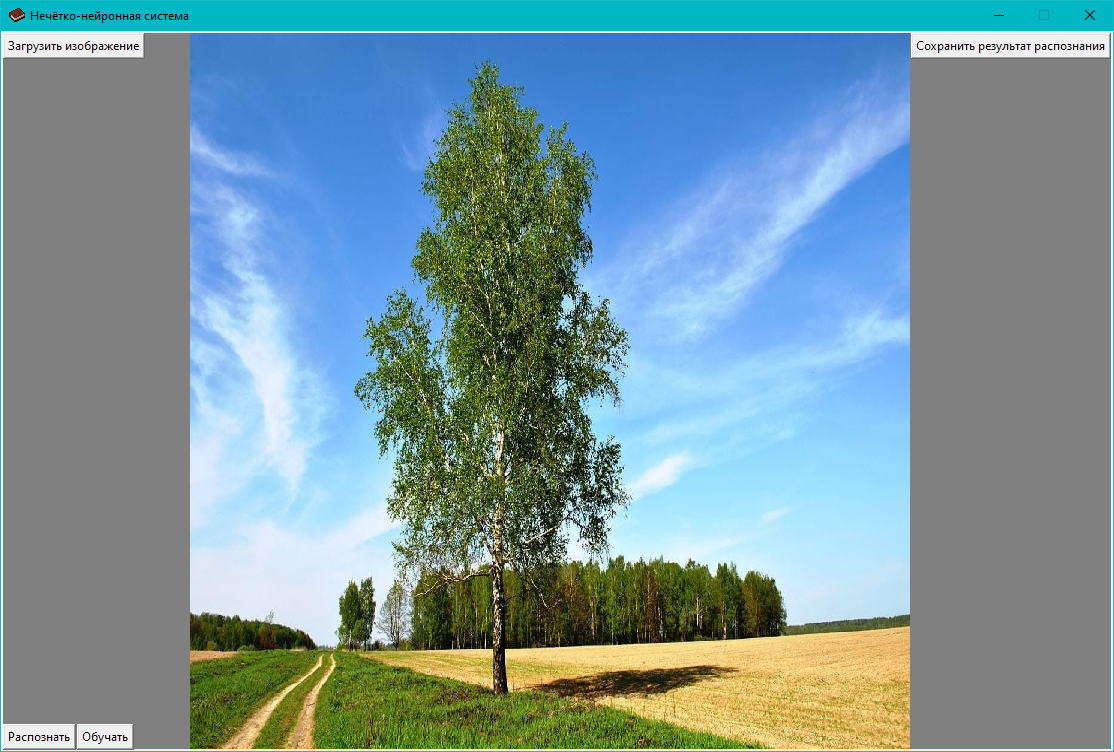
\includegraphics[width=1\linewidth]{systemtest_responce15}}
\caption{Интерфейс с изображением берёзы}
\label{systemtest_responce15:image}
\end{figure}

На рисунке \ref{systemtest_responce16:image} изображение берёзы было обработано по модели ''Белый''.

\begin{figure}[H]
\center{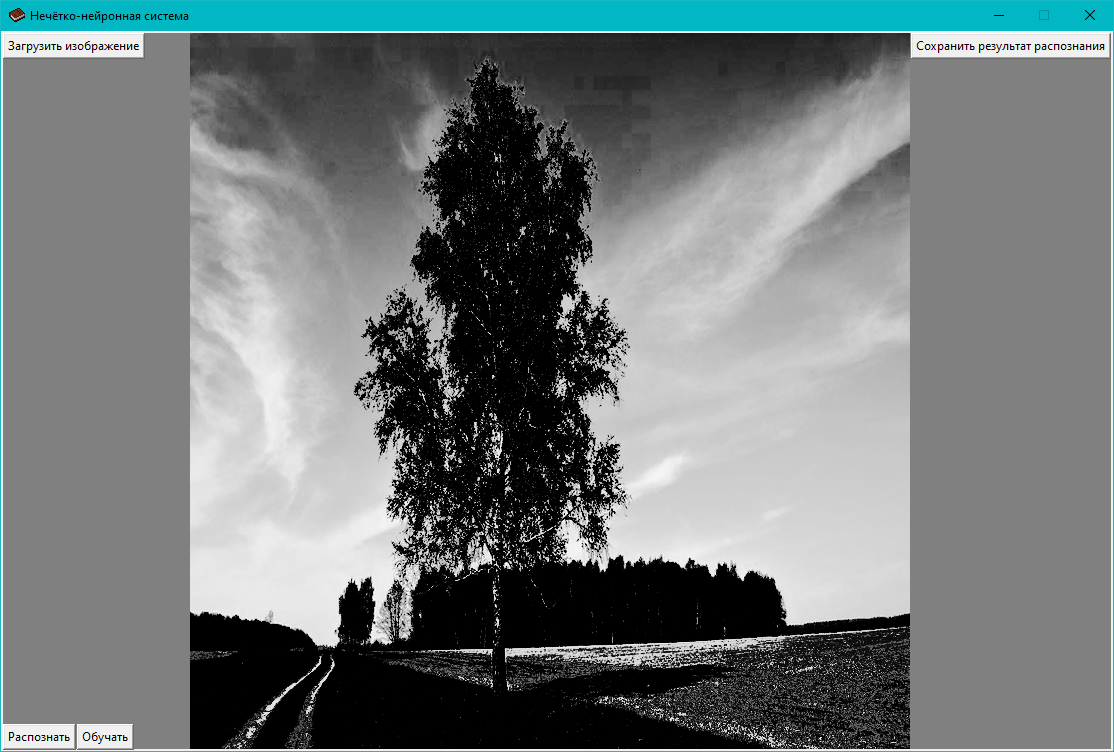
\includegraphics[width=1\linewidth]{systemtest_responce16}}
\caption{Распознанныйе объекты на изображении берёзы}
\label{systemtest_responce16:image}
\end{figure}
   \section*{ЗАКЛЮЧЕНИЕ}
\addcontentsline{toc}{section}{ЗАКЛЮЧЕНИЕ}

В заключение, проект по созданию интеллектуальной системы распознавания объектов по цветовым характеристикам на основе нечётких нейронных сетей демонстрирует значительный прогресс в области компьютерного зрения. Эта разработка не только подтверждает возможности искусственного интеллекта и машинного обучения в решении сложных задач, но и открывает новые перспективы для их применения в различных сферах жизнедеятельности человека.

Использование адаптивных нечётких нейронных сетей позволяет системе эффективно адаптироваться к изменяющимся условиям и обеспечивает высокую точность распознавания объектов. Таким образом, данное приложение может стать незаменимым инструментом в медицинской диагностике, обеспечении безопасности и других ключевых областях.

Проект также иллюстрирует важность синергии между технологическими инновациями и потребностями общества. Результаты, полученные в ходе работы над проектом, могут служить основой для дальнейших исследований и разработок, направленных на улучшение качества жизни и безопасности людей.

Таким образом, проект подчёркивает роль искусственного интеллекта как ключевого фактора в продвижении научно-технического прогресса и открывает новые горизонты для инновационных исследований в будущем.

Основные результаты работы:

\begin{enumerate}
\item Проведен анализ предметной области. Выявлена необходимость использовать язык Python и билиотеки MATLAB;
\item Разработана концептуальная модель приложения. Разработана модель данных системы. Определены требования к системе;
\item Осуществлено проектирование приложения. Разработана архитектура нейронной сети и базы данных. Разработан пользовательский интерфейс приложения;
\item Реализовано и протестировано приложение. Проведено модульное и системное тестирование.
\end{enumerate}

Все требования, объявленные в техническом задании, были полностью реализованы, все задачи, поставленные в начале разработки проекта, были также решены.

Готовый рабочий проект представлен приложением. 

}\fi
\addcontentsline{toc}{section}{СПИСОК ИСПОЛЬЗОВАННЫХ ИСТОЧНИКОВ}

\begin{thebibliography}{13}

    \bibitem{python} Лутц, М. Изучаем Python, 5-е издание / М. Лутц. – Санкт-Петербург : Питер, 2019. – 1584 с. – ISBN 978-5-4461-0705-9. – Текст~: непосредственный.
    \bibitem{deeplearning} Гудфеллоу, И., Бенджио, Ю., Курвилль, А. Глубокое обучение / И. Гудфеллоу, Ю. Бенджио, А. Курвилль. – Москва : ДМК Пресс, 2017. – 652 с. – ISBN 978-5-97060-487-9. – Текст~: непосредственный.
    \bibitem{neuralnetworks} Хайкин, С. Нейронные сети: полный курс, 2-е издание / С. Хайкин. – Москва : Вильямс, 2018. – 1104 с. – ISBN 978-5-8459-2101-0. – Текст~: непосредственный.
    \bibitem{fuzzylogic} Росс, Т. Дж. Нечеткая логика с приложениями в инженерных науках / Т. Дж. Росс. – Москва : Мир, 2016. – 800 с. – ISBN 978-5-03-004474-5. – Текст~: непосредственный.
    \bibitem{machinelearning} Мерфи, К. Машинное обучение: вероятностный подход / К. Мерфи. – Москва : ДМК Пресс, 2018. – 704 с. – ISBN 978-5-97060-212-7. – Текст~: непосредственный.
    \bibitem{pythonmachinelearning} Рашка, С., Мирджалили, В. Python и машинное обучение / С. Рашка, В. Мирджалили. – Москва : ДМК Пресс, 2018. – 418 с. – ISBN 978-5-97060-310-0. – Текст~: непосредственный.
    \bibitem{tensorflow} Жолковский, Е. К. TensorFlow для профессионалов / Е. К. Жолковский. – Москва : ДМК Пресс, 2019. – 480 с. – ISBN 978-5-97060-746-7. – Текст~: непосредственный.
    \bibitem{keras} Чоллет, Ф. Глубокое обучение на Python / Ф. Чоллет. – Москва : ДМК Пресс, 2018. – 304 с. – ISBN 978-5-97060-409-1. – Текст~: непосредственный.
    \bibitem{fuzzysystems} Клейн, Р. Нечеткие системы в Python / Р. Клейн. – Москва : ДМК Пресс, 2020. – 320 с. – ISBN 978-5-97060-758-0. – Текст~: непосредственный.
    \bibitem{advancedpython} Бейдер, Д. Python Tricks: A Buffet of Awesome Python Features / Д. Бейдер. – Москва : ДМК Пресс, 2021. – 300 с. – ISBN 978-5-97060-999-7. – Текст~: непосредственный.
    \bibitem{practicalml} Герон, О. Практическое машинное обучение с Scikit-Learn и TensorFlow / О. Герон. – Москва : ДМК Пресс, 2019. – 572 с. – ISBN 978-5-97060-524-1. – Текст~: непосредственный.
    \bibitem{neuralnetspython} Нильсен, М. Нейронные сети и глубокое обучение / М. Нильсен. – Москва : ДМК Пресс, 2021. – 250 с. – ISBN 978-5-97060-777-1. – Текст~: непосредственный.
    \bibitem{fuzzypy} Джеймс, Д. Нечеткие системы и Python: практическое руководство / Д. Джеймс. – Москва : ДМК Пресс, 2022. – 340 с. – ISBN 978-5-97060-888-4. – Текст~: непосредственный.

\end{thebibliography}

\ifВКР{\appendix{Представление графического материала}

Графический материал, выполненный на отдельных листах,
изображен на рисунках А.1--А.\arabic{числоПлакатов}.
\setcounter{числоПлакатов}{0}

\renewcommand{\thefigure}{А.\arabic{figure}} % шаблон номера для плакатов

\begin{landscape}

\begin{плакат}
    
\includegraphics[width=0.82\linewidth]{плакат1.png}
    \заголовок{Сведения о ВКРБ}
    \label{pl1:image}      
\end{плакат}

\begin{плакат}
    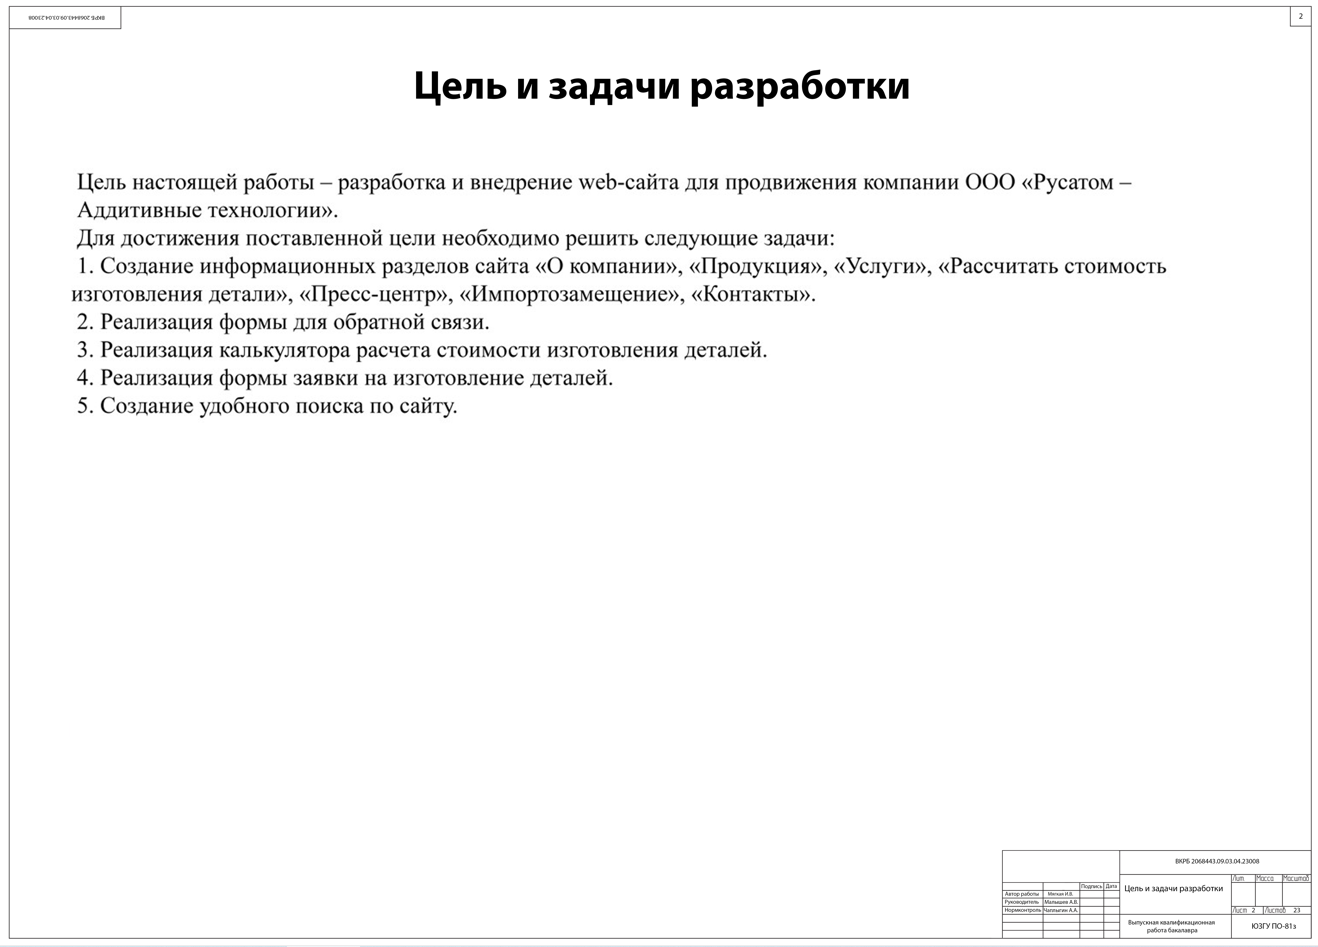
\includegraphics[width=0.82\linewidth]{плакат2.png}
    \заголовок{Цель и задачи разработки}
    \label{pl2:image}      
\end{плакат}

\begin{плакат}
    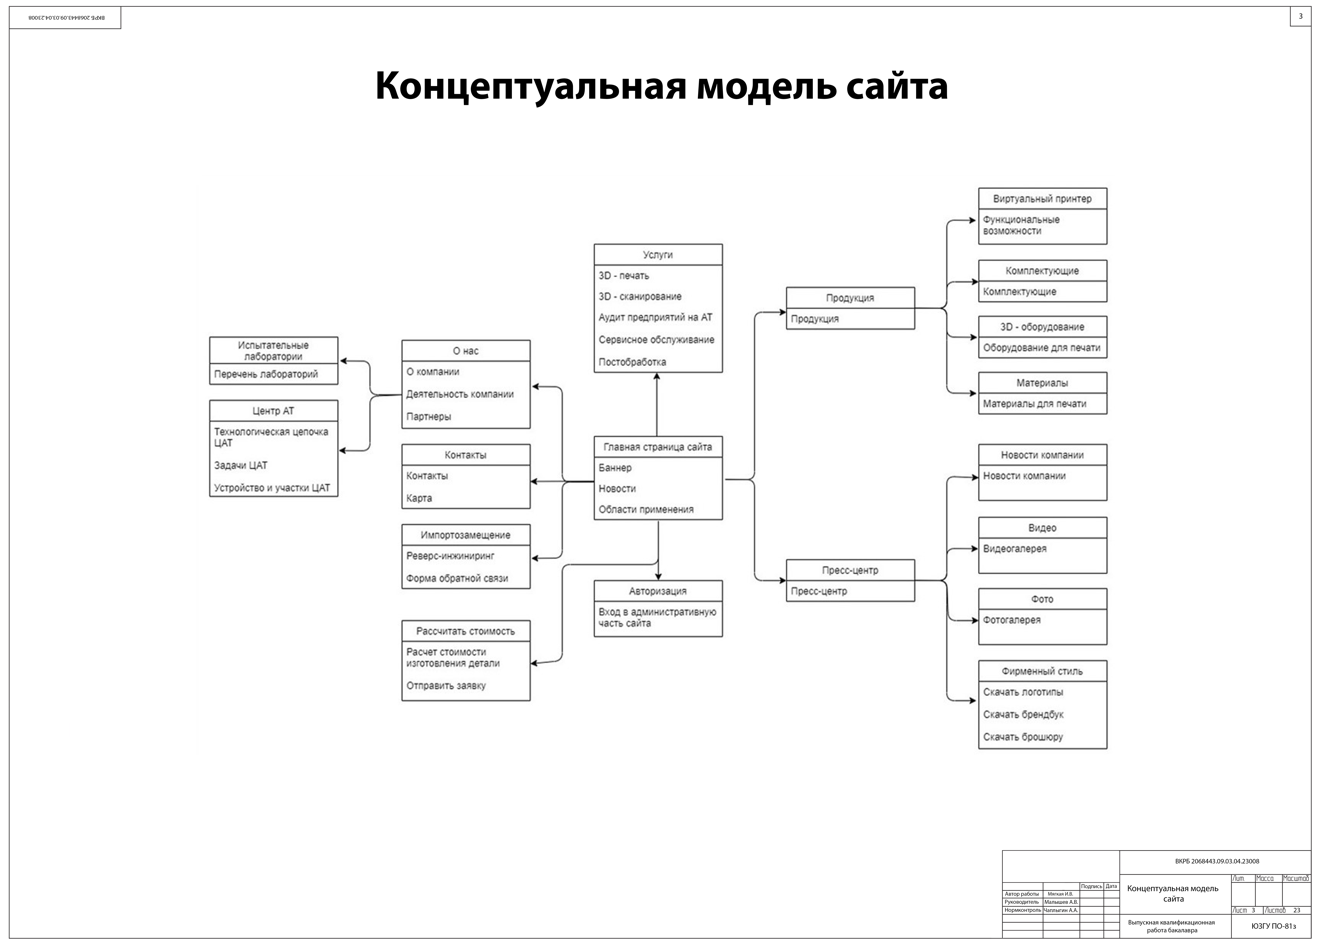
\includegraphics[width=0.82\linewidth]{плакат3.png}
    \заголовок{Концептуальная модель сайта}
    \label{pl3:image}      
\end{плакат}

\begin{плакат}
    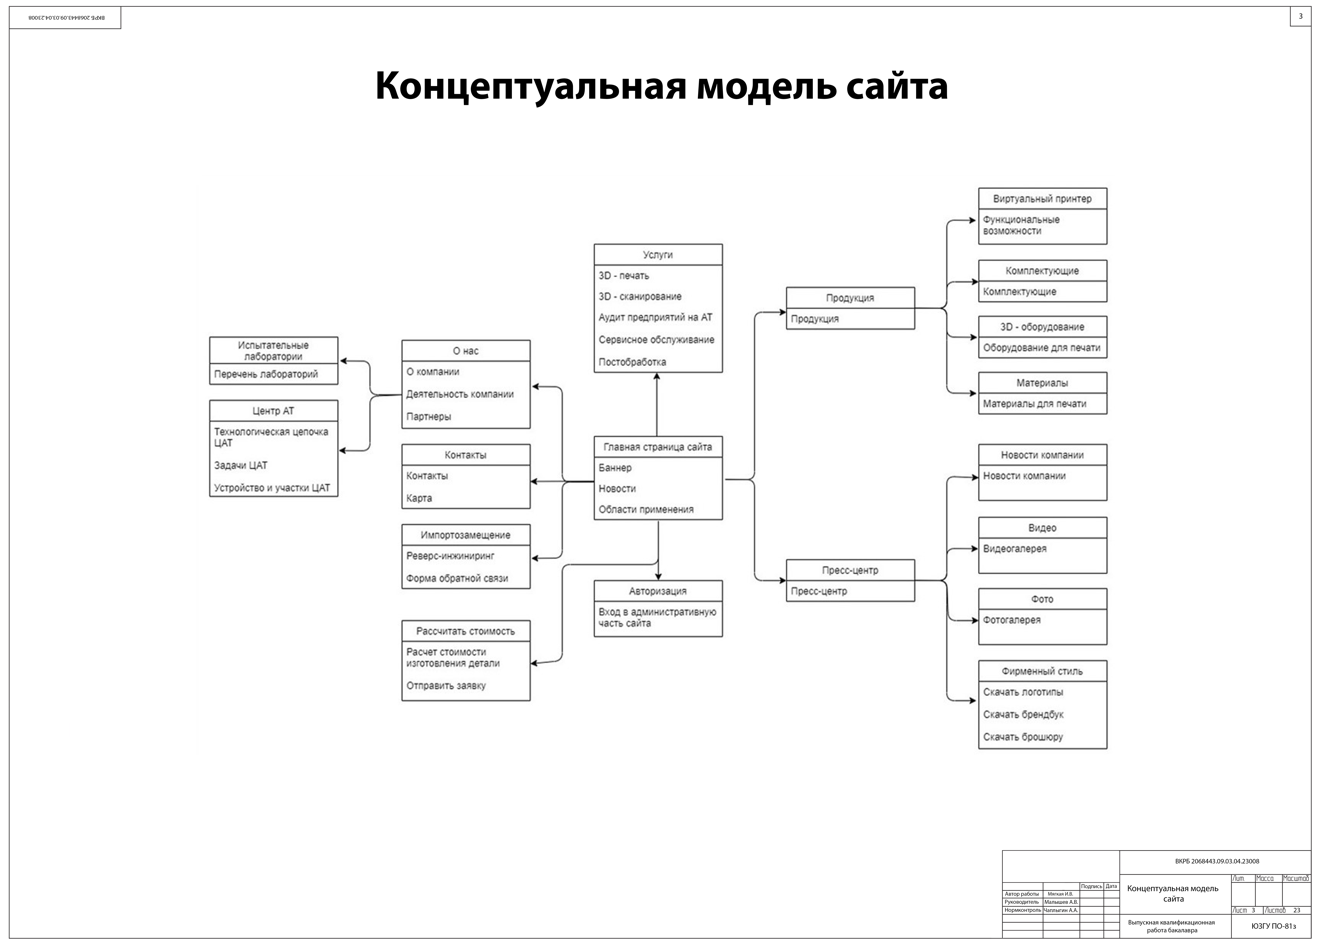
\includegraphics[width=0.82\linewidth]{плакат3.png}
    \заголовок{Еще плакат}
    \label{pl4:image}      
\end{плакат}

\end{landscape}
}\fi
\ifПрактика{}\else{\appendix{Фрагменты исходного кода программы}

main.tex
\lstinputlisting[language=Tex, frame=none]{main.tex}

ТехПроект.tex
\lstinputlisting[language=Tex, frame=none]{ТехПроект.tex}

\ifВКР{
\newpage
\addcontentsline{toc}{section}{На отдельных листах (CD-RW в прикрепленном конверте)}
\begin{center}
\textbf{Место для диска}
\end{center}
}\fi
}\fi
\end{document}
